% 公立はこだて未来大学 卒業論文 テンプレート ver1.50
% (c) Junichi Akita (akita@fun.ac.jp), 2003.10.31
% update by N.T.,  2004.11.10
%
\documentclass{funthesis}
%\documentclass[english]{funthesis} % use [english] option for English style

%\usepackage{graphicx} % 図(EPS形式)を本文中で読み込む場合はこれを宣言
\usepackage[dvipdfmx]{graphicx}
\graphicspath{{./img/}}
\usepackage{here}
 \usepackage{url}

% この部分に,タイトル・氏名などを書く.
% タイトルなどの定義の始まり
\jtitle{Leap Motionによる教育をインタラクティブにする\\システムの提案\\
%--- 一二三四五六七八九十 ---
}  % 論文の和文タイトル
%
\etitle{Interactive system for education by leap motion sensor
}% 論文の英文タイトル
%q
\htitle{Interactive system for education by leap motion sensor}   % ヘッダー用の論文の短縮英文タイトル
%     必ず1行に収まるように英文タイトルを短縮する.
%
\jauthor{一ノ瀬 智太}     % 氏名(日本語)
\eauthor{Tomohiro Ichinose }   % 氏名(英語)
\jaffiliciation{情報アーキテクチャ学科} % 所属学科名(日本語)
\eaffiliciation{Department of Media Architecture} % 所属学科名(英語)
\studentnumber{1012211}   % 学籍番号
\jadvisor{美馬 義亮}    % 正指導教員名(日本語)
%\jcoadvisor{副指導 教員} % 副指導教員(日本語)がいる場合は
                        % コメントアウトし名前を書く
                        % 副指導教員がいない場合は,ここは削除しても可
\eadvisor{Yoshiaki Mima}  % 正指導教員名(英語)
%\ecoadvisor{Prof. Coadvisor}   % 副指導教員(英語)がいる場合は
                         % コメントアウトし名前を書く
                         % 副指導教員がいない場合は,ここは削除しても可
\jdate{平成28年1月29日}    % 論文提出日   (日本語)
\edate{January 29, 2016}     % 論文提出年月 (英語)
% タイトルなどの定義の終わり

\begin{document}

%--------------------------------------------------------------------
\maketitle       % タイトルページを作成

%--------------------------------------------------------------------
% 英文概要(250語程度)
\begin{eabstract}
Teachers use a blackboard and chalk in the classroom. Students has been used pencil and notebook. However, classes that use a personal computer and tablet devices have been introduced in recent years. Teacher make the documentation for classes by PC. And Teacher projected it for the projector. The form is being spreaded what the teacher is able to send information to a student along it. Also, new devices has introduced. They are Leap Motion and Ring, Smart Watch. Thus, user come to  not push keyboard and wear devices. It is that the exchanges of the information from a teacher to a student are unilateral to be common when I compared the recent school education with the conventional thing. Teachers talk about classes with platform, students are learning to hear it. In this study, I assumed that use of leap motion when implement application which capable input method. It is not mouse and keyboard. In this study, the purpose is to implement an application which capable this function, and evaluate usefulness.
\end{eabstract}

% 英文キーワード(5個程度をコンマ(,)で区切って羅列する)
\begin{ekeyword}
Interaction, Leap Motion, Gesture
\end{ekeyword}

%--------------------------------------------------------------------
% 和文概要(400字程度)
\begin{jabstract}
学校教育の場において教師は黒板とチョークを使い, 学生は鉛筆やノートを使った授業が主流であった. しかし, 近年ではパーソナルコンピュータやタブレット端末を使った授業が取り入れられている. 例えば, 教師は授業の資料をPCで作成し, プロジェクターなどで投影する. それに沿って教師は学生へ情報を発信するというような形態が広まりつつある.  また, 新しいデバイスが登場している. Leap MotionやRing, スマートウォッチなどが例である. これによりキーボードを叩かずに入力操作を行ったり, デバイスを身につけるという変化が起こっている. 近年の学校教育を従来のものと比較した際に共通することは, 教師から学生への情報のやり取りが一方的なことである. 教師は授業に関することを教壇で話し, 学生はそれを聞いて学習する. 本研究では, Leap Motionを使うことを前提として, マウスやキーボードにない入力方法でメッセージを発信するアプリケーションを実装する. そのとき提案するアプリケーションが話者の邪魔をしたり, 話者の応答がないものであってはならない. 本研究では, これらを踏まえたアプリケーションを実装し,その有用性を評価することを目的とする. 

\end{jabstract}

% 和文キーワード(5個程度をコンマ(,)で区切って羅列する)
\begin{jkeyword}
双方向性, Leap Motion, ジェスチャー
\end{jkeyword}

%--------------------------------------------------------------------
\tableofcontents % 目次を作成


% 本文のはじまり
%--------------------------------------------------------------------
\chapter{序論} % 章のタイトル
%\chapter{Introduction} % sample of English style

% \includegraphics[width=??cm]{hoge.eps} % 図(EPS形式)を読み込む場合

\section{背景} % sectionのタイトル

% 以下に背景,関連する環境,状況,技術に関する概要を記述.

%ここはneeds
学制百年史\cite{A1} によると日本における大学の誕生は明治時代に遡る. これらは一斉授業の場において,教師は知識を与え学生はそれを吸収するというモデルに基づいている. こうした場において, 一部の学生には頬杖をついたり, 居眠りをしたりすることなどが散見される. その原因として, 日々の生活の疲れだけでなく, 教師の説明が理解できず, 授業についていけないなどのストレスが挙げられる. こうした学生には他の学生に比べて学習意欲が低下しているといえる. 大学のゼミにおいても同じような状況があるといえる. 話し手が進捗報告や自分の考えを一方的に話し, 聞き手はそれに耳を傾ける. 近年では, Leap MotionやRing, スマートウォッチなどの新しいデバイスが登場している. その結果, 今までマウスやキーボードで入力する方法以外にも, ジェスチャーを使って入力したりPCを操作できるようになった. また, 学校内でのLANや学外でのロボットコンテストなどが普及してきており,  PCやタブレット端末などが教育でも使われるようになってきたといえる. 

\section{研究目標}
本研究では, 授業中やゼミの中で情報のやりとりが一方的に行われている問題に着目した. この問題を解決するために教師や発表者である話し手と, 話を聞く聞き手との間に双方向性をもたせ,  対話的な授業運営, ゼミの進行を図ることを研究目標とする. その方法として, Leap Motionというセンサが手や指の位置, 方向, 曲げ, ジェスチャー等を検知できるセンサを用いて, 双方向性を実現するアプリケーションを実装することを目的とする. 具体的には学生が授業中に抱いている「大きな声で話してほしい」や「もう一度説明してほしい」などのメッセージをLeap Motionで入力し,教師に伝えるということをめざす. この時, 話し手には話の邪魔をしないことや話し手が応答があるようにすることを前提とし, これを満たすアプリケーションの提案を目指す. 

%もっと何をしたいのかを明確に記述する
%追記 ” 授業に大きな影響を与えることなく ” 

%\section{研究目標}


%--------------------------------------------------------------------
%\chapter{問題設定・研究アプローチ} % 章のタイトル
%\chapter{Introduction} % sample of English style

%\section{問題設定}
% \includegraphics[width=??cm]{hoge.eps} % 図(EPS形式)を読み込む場合

%言い回しが長くならないようにする
%本研究での問題は一斉授業の場において双方向性を実現し, 学習意欲の向上を目指す. Leap Motion というセンサが手や指の動きを検知し入力操作を行い, その時に音を立てないのでこれを使用する. 本研究での一斉授業の場の位置付けとして, 教師と学生の双方がパーソナルコンピュータを使用していることを想定する. 具体的な例として, 教師はパーソナルコンピュータで資料をプロジェクターに投影しながら授業を行い, 一方, 学生はメモをとったり課題に取り組むために使用しているものとする.

% 以下に現状の問題・研究アプローチを記述.

%\section{研究アプローチ}
%ここでは実際のアプリケーションを使うときのシナリオを記述する. まず, 実際の授業や中で学生は「大きな声で話してほしい」や「もう一度説明してほしい」といった感情を抱く. これらの感情を Leap Motion を使ったアプリケーションで発信する. 
%具体性が欲しい

%--------------------------------------------------------------------
\chapter{関連研究}
ここでは対話的授業運営の関連研究としてクリッカーを, 意思決定ツールとしてサイボウズLiveを取り上げる.
%グループウェアで検索してまだないか調べる

%コンセプトを絵にする
\section{クリッカー }
双方向性授業の実現としてクリッカー\cite{A5} を用いた事例がある. 武田氏\cite{A2} のクリッカー(授業応答システム)とは赤外線リモコンによる学生解答システムである. 授業中に教師が問題を出し, 学生がクリッカーを用いて解答するというものである. 集計結果は瞬時にグラフ化され, スクリーンに表示される. また, 投票は匿名で行われる. クリッカーを用いた結果として,「役に立つ」という問いに対して「役に立つ」と答えた学生が 6 割を上回り,「勉強する気になったか」という問いに対しては「やる気が出た」という学生が 7 割を上回っている.
%どのように使うのかを記述
%本システムとの違いを描く
%画像の挿入
\begin{figure}[H]
  \begin{center}
  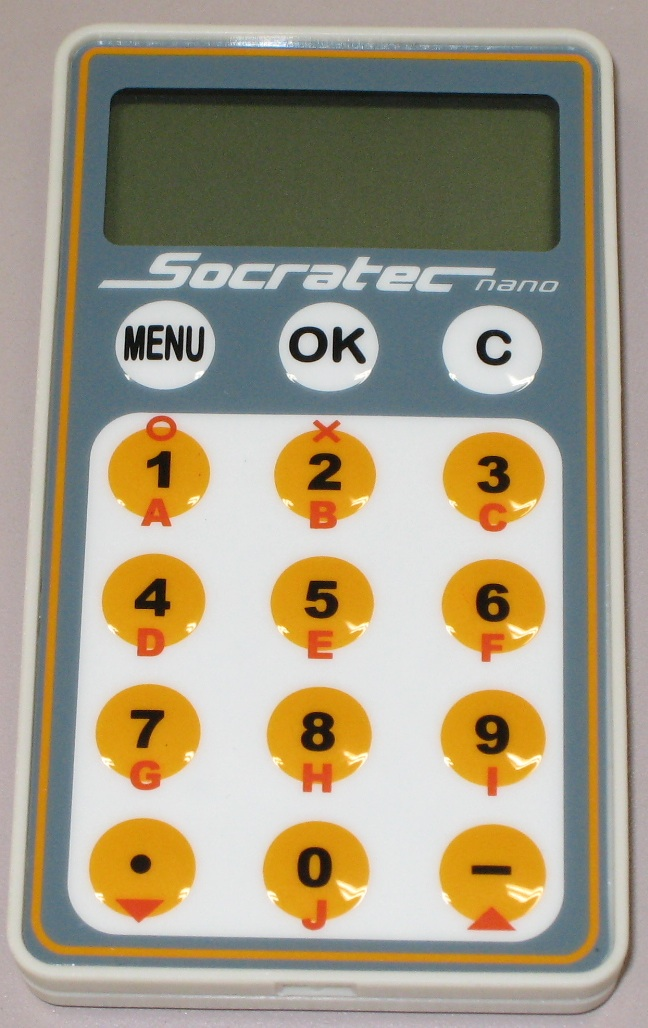
\includegraphics[width=50mm]{./img/clicker.jpg}
  \end{center}
  \caption{クリッカー}
  \label{senni1}
 \end{figure}

\subsection{提案するシステムとの違い}
クリッカーは教師が出した問題に対して学生が解答するためのツールであり, 学生側がメッセージを発信するツールではない.  先生からの選択肢に答えるだけでなく, 授業に対するストレスや評価などを自然な形で発信することが重要だと考えた. 


\section{サイボウズLive \cite{A3} }

%サイボウズ
%http://products.cybozu.co.jp/office/
%サイボウズlive
%https://live.cybozu.co.jp/overview.html

%サイボウズ社が開発した意思決定ツール
%主な機能
%導入事例とか...

サイボウズLive(\ref{cybozu})はサイボウズ社が開発した意思決定ツールである. 
主な機能として、以下の5つが紹介されている.
\begin{itemize}
 \item タイムライン:メンバーに聞きたいこと、伝えたいことを書く
 \item 掲示板:掲示板のコメント欄でメンバーとディスカッションする
 \item イベント:プロフェクトのイベントやスケジュールを登録・共有できる
 \item ToDoリスト:メンバーとToDoを共有できる
 \item 共有フォルダ:1グループにつき1Gバイトまで無料でファイルを保存可能
\end{itemize}
また, チャット機能の利点は以下の3つが紹介されている.\\
 1つ目は, PCでもスマートフォンでもメッセージがすぐ届く点である. サイボウズLiveのチャット機能はPCだけでなく, スマートフォンでも使うことできる. 投稿したコメントは相手の画面にただちに用事されるので, オンラインのミーティングがスムーズに行える. \\
 2つ目は,  複数人でも1対1でもチャットが出来る点である. 複数人のメンバーを指定して, チャットスペースを作成できる. また, サイボウズLive上で知人と繋がると, 自動的に1対1のチャットスペースが作成されるので, 簡単にチャットのやりとりをスタートできる. \\
 3つ目は,  グループ機能と併用すれば, 情報の整理が楽になるという点である. チャットのやりとりで決定したことは, 先に記述したToDoリストに登録しておくことができる. \\
%画像の挿入
\begin{figure}[H]
 \begin{center}
  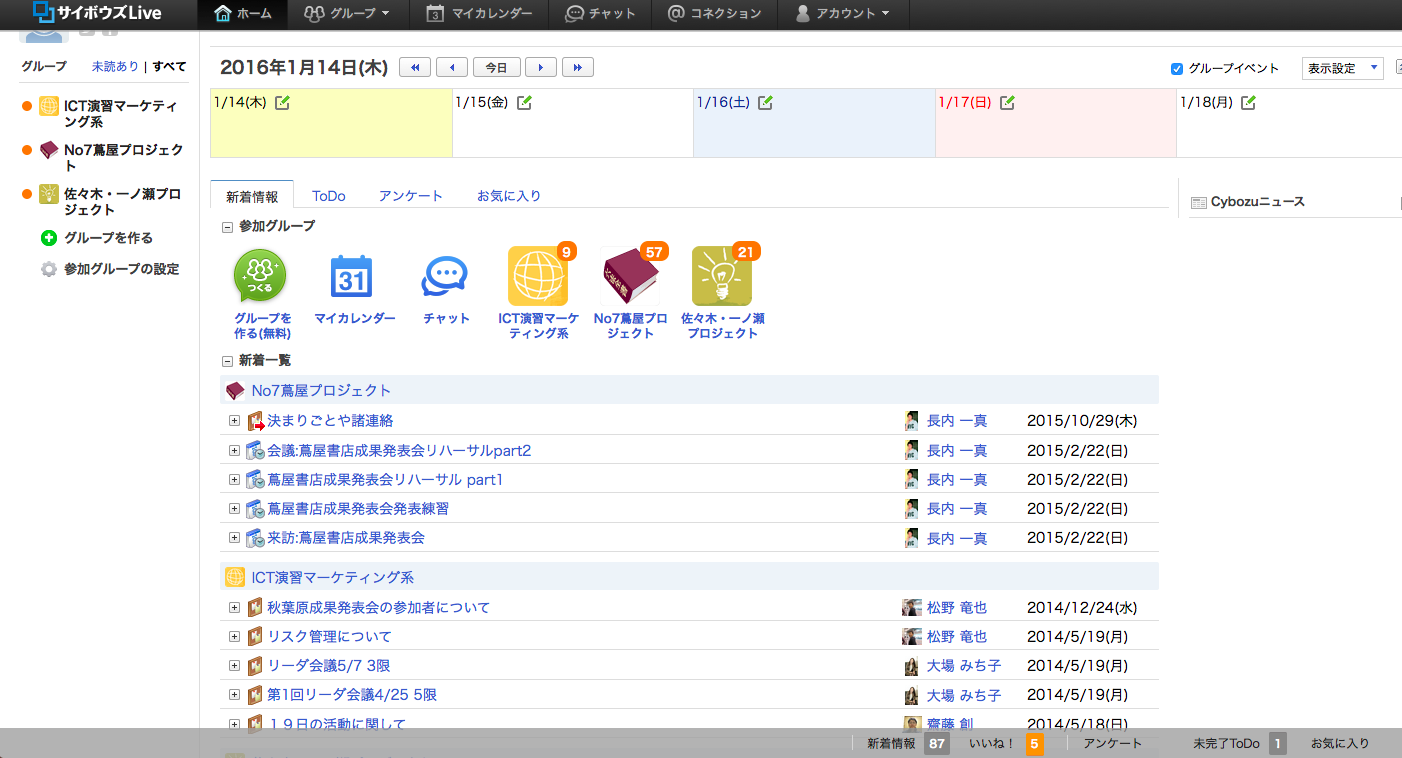
\includegraphics[width=110mm]{./img/cybozulive.png}
 \end{center}
 \caption{サイボウズLive}
 \label{cybozu}
\end{figure}

%本システムとの違いを描く
\subsection{提案するシステムとの違い}
本システムとの違いは1つは入力方法である. 提案するシステムは入力装置としてLeap Motionを使っている. 対してサイボウズLiveはスマホやPCを使って入力する. キーボードやマウスを使って入力するものであり, 手や指の動きで入力操作はできない. 

%--------------------------------------------------------------------
\chapter{提案するシステムの概要}

%この章では,提案する理論,仮説,モデル,アルゴリズム,方法論,実装のなどの説明を行う
提案するシステムは、授業やゼミ等で聞き手が話し手にメッセージを発信するための意思決定ツールである.  例えばゼミで話し手の声が小さかったり, 説明がわかりにくかったとする.  このとき聞き手側が本システムを使用し, 「大きな声で話してほしい」や「もう一度説明してほしい」などのメッセージを発信する. その発信を話し手が気づき, 応答するという状況を起こすために製作した. 

\section{提案するシステムの特徴}
%この言語の特徴は,..であり,...という従来にない長所をもつ.
%このアプリケーションの特徴は、クライアント側はLeap Motionを使ってリアルタイムに入力操作を行い、サーバー側に反映するという長所がある.
%このアプリケーションの主な特徴は, Leap Motionを使ってリアルタイムに入力操作を行うことである.
%自分が発信したいメッセージを選択するだけ
%ソケット通信を使って通信を行う。お互いのPCがインターネットに接続されていなければならない。
\begin{figure}[H]
  \begin{center}
  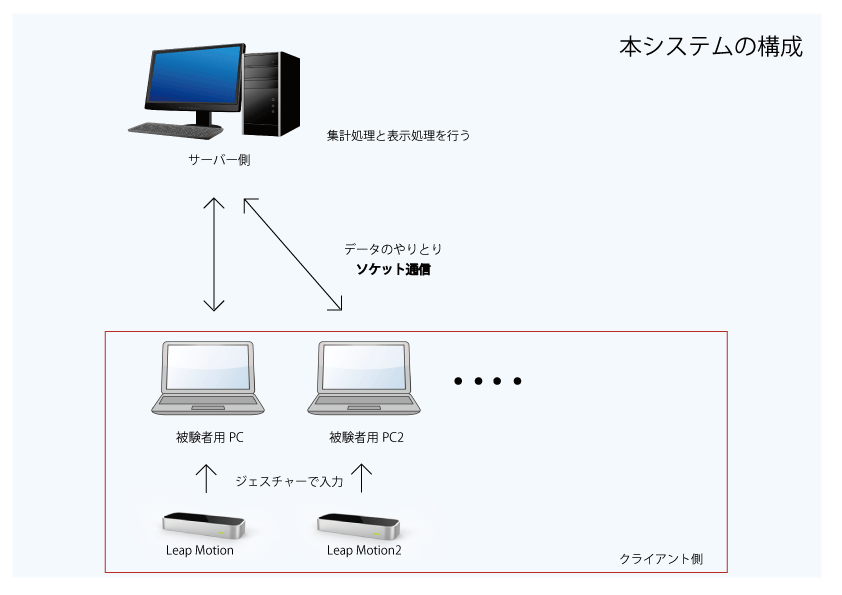
\includegraphics[width=120mm]{./img/kosei2.png}
  \end{center}
  \caption{本システムの構成図}
  \label{kosei2}
 \end{figure}

%ユーザ視点での特徴を丁寧に箇条書き
%機能で説明する
このアプリケーションの主たる特徴は, 2つある.\\
 1つ目は, Leap Motionで読み取る4つのジェスチャーを使い, リアルタイムに入力操作を行うことである. \\
%そもそもの経緯がLeap Motionを使うことにあった
 2つ目は, クライアント側とサーバー側の二つのプログラムに分かれていることである. このアプリケーションでは, クライアント側とサーバー側間のデータを送受信する手段として, ソケット通信を行った. \\
 このアプリケーションの機能は以下のものがある.
\begin{itemize}
 \item ジェスチャーを使ってメッセージを発信する機能
 \item 発信するメッセージに重みをつける機能
 \item 発信されたデータを集計する機能
\end{itemize}

\subsubsection{メッセージの種類}
このシステム上でやりとりするメッセージの種類は以下の9つである
\begin{itemize}
 \item 大きな声で
 \item 頑張れ!
 \item もう一度説明して
 \item 面白い!
 \item トイレに行きたい
 \item わかった
 \item かっこいい!
  \item ゆっくり話して
 \item わからない
\end{itemize}


\section{クライアント側プログラムの役割}
クライアント側プログラムは, 聞き手が発信したいメッセージを発信するためのものである.  聞き手はLeap Motionを使い, メッセージの発信を行う. 

\subsubsection{メッセージを発信する手順}

クライアント側がメッセージを発信する際, 全ての手順をLeap Motionで読み取ったジェスチャーで行うという特徴がある. ジェスチャーについては後に続くLeap Motionの評価に説明する. このように製作した理由は, マウスやキーボードなどの入力装置との差別化を行うためである. 聞き手がメッセージを送信するために行う手順は, 以下の3つある. 
\begin{enumerate}
 \item ジェスチャーを行い, 入力方法を決める(図\ref{senni1}). 
 \item ジェスチャーでメッセージの選択を行う(図\ref{senni2}). 
 \item ジェスチャーの回数で, メッセージに重みをつける(図\ref{senni3}). 
\end{enumerate}

まず, 画面遷移1でジェスチャーを行い, 入力方法を決める. 例えば, このときLeap Motion上で円を描くサークルジェスチャーを行った場合, このジェスチャーがメッセージを発信するまでの入力方法になる. 
次に, ジェスチャーでメッセージの選択を行う. 30秒間の時間が設けてあり, ユーザーはこの時間内に自分が発信したいメッセージを選択する. 最後に選択されていたメッセージがサーバー側へ送信する値になる. %このときジェスチャーをするときの指の本数で選択される仕様になっている. 
最後に, ジェスチャーでメッセージに重みをつける. この段階でも30秒の値が設けてある. ジェスチャーを行った回数で, 自分がどれだけメッセージを伝えたいか発信するメッセージに重みをつけることができる. この回数が次に紹介する各ジェスチャーの値に相当し, 値の大小でサーバー側プログラムの描写が変わる. 

\begin{figure}[H]
  \begin{center}
  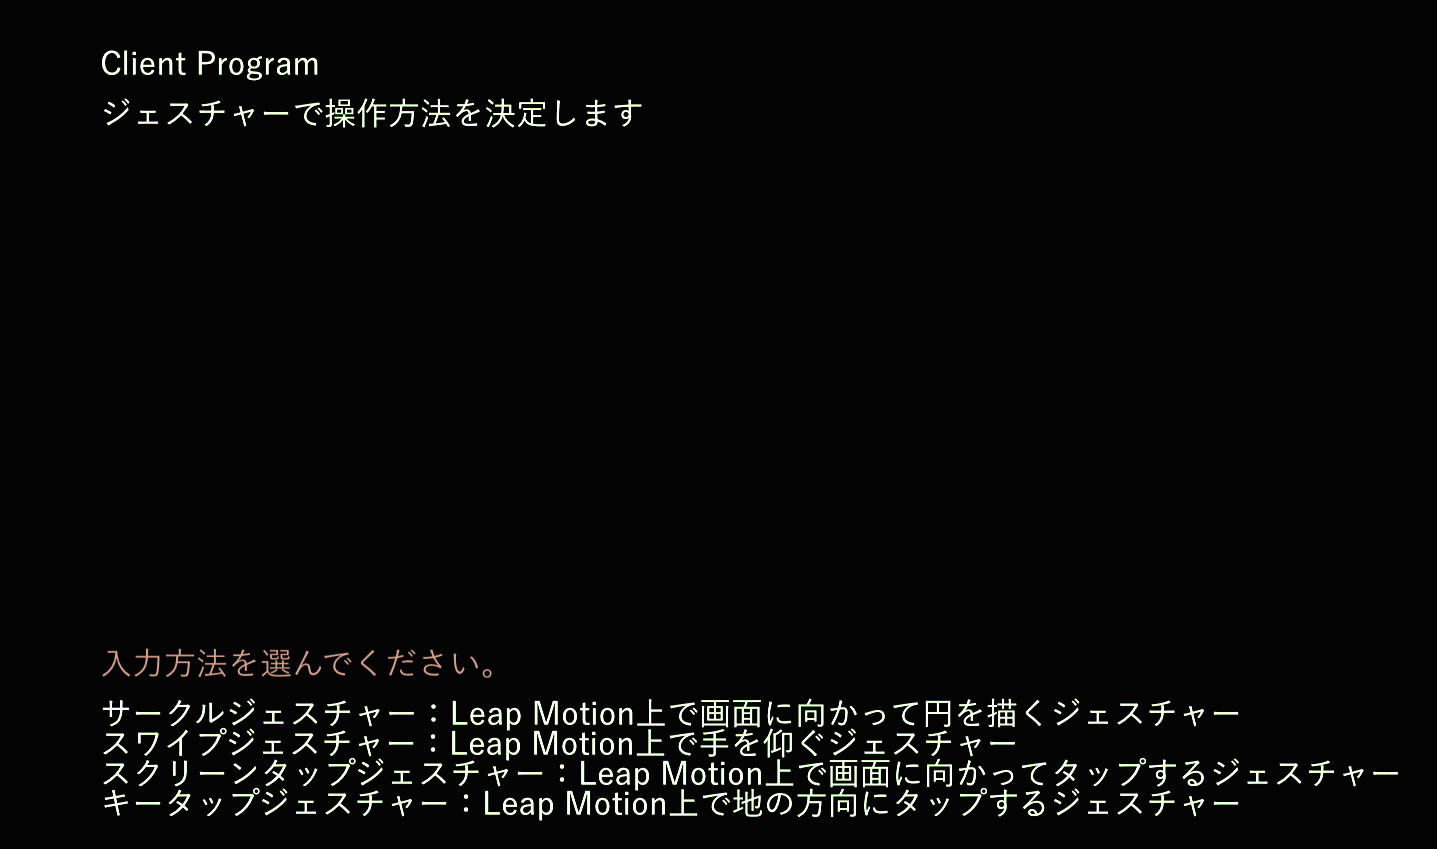
\includegraphics[width=120mm]{./img/clseni1.png}
  \end{center}
  \caption{画面遷移1}
  \label{senni1}
 \end{figure}
 
 \begin{figure}
  \begin{center}
  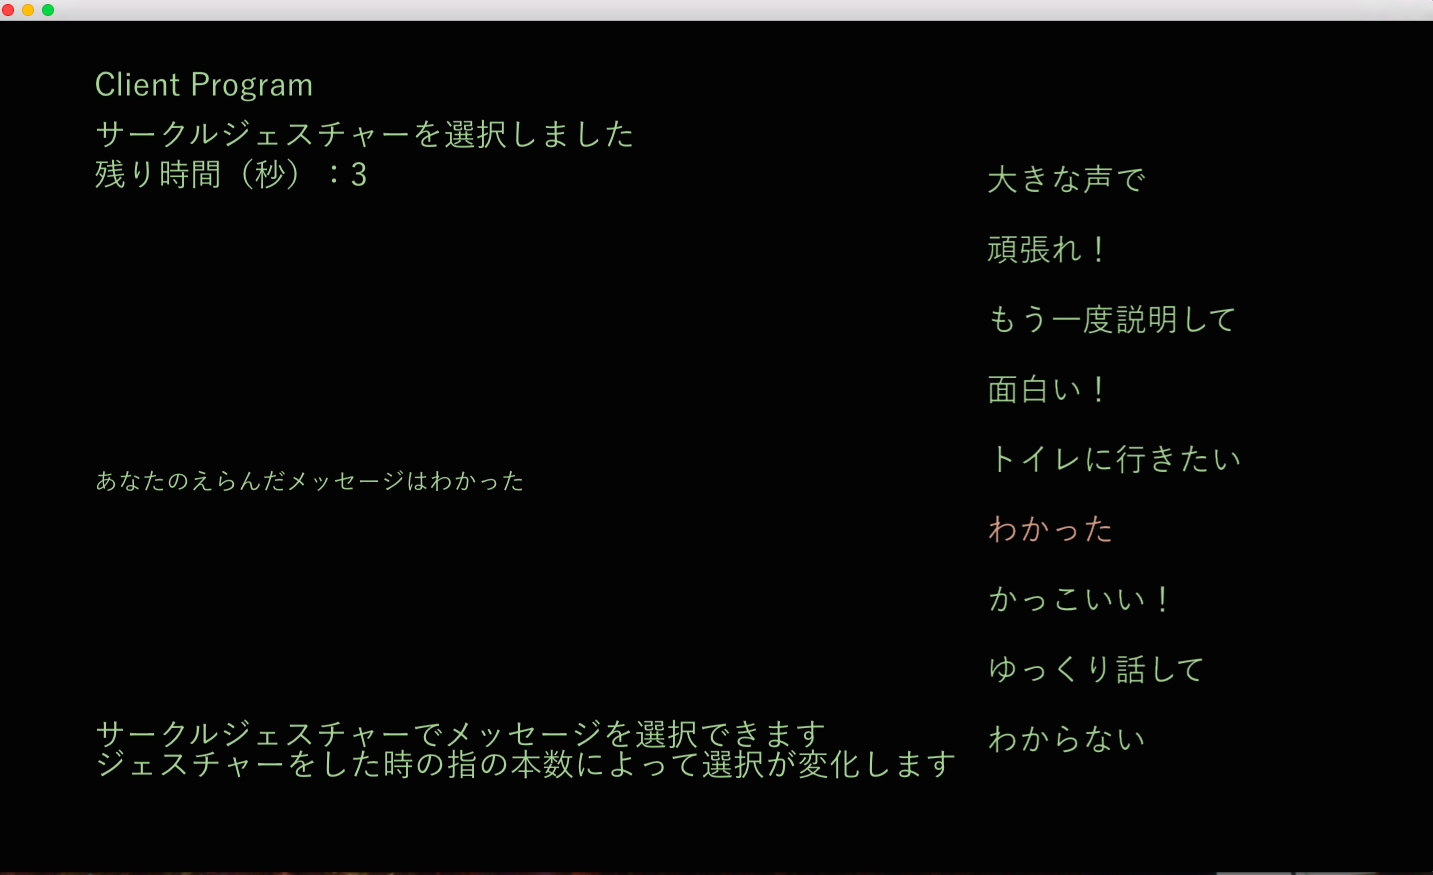
\includegraphics[width=120mm]{./img/clseni2.png}
  \end{center}
  \caption{画面遷移2}
  \label{senni2}
  \end{figure}
   \begin{figure}
  \begin{center}
  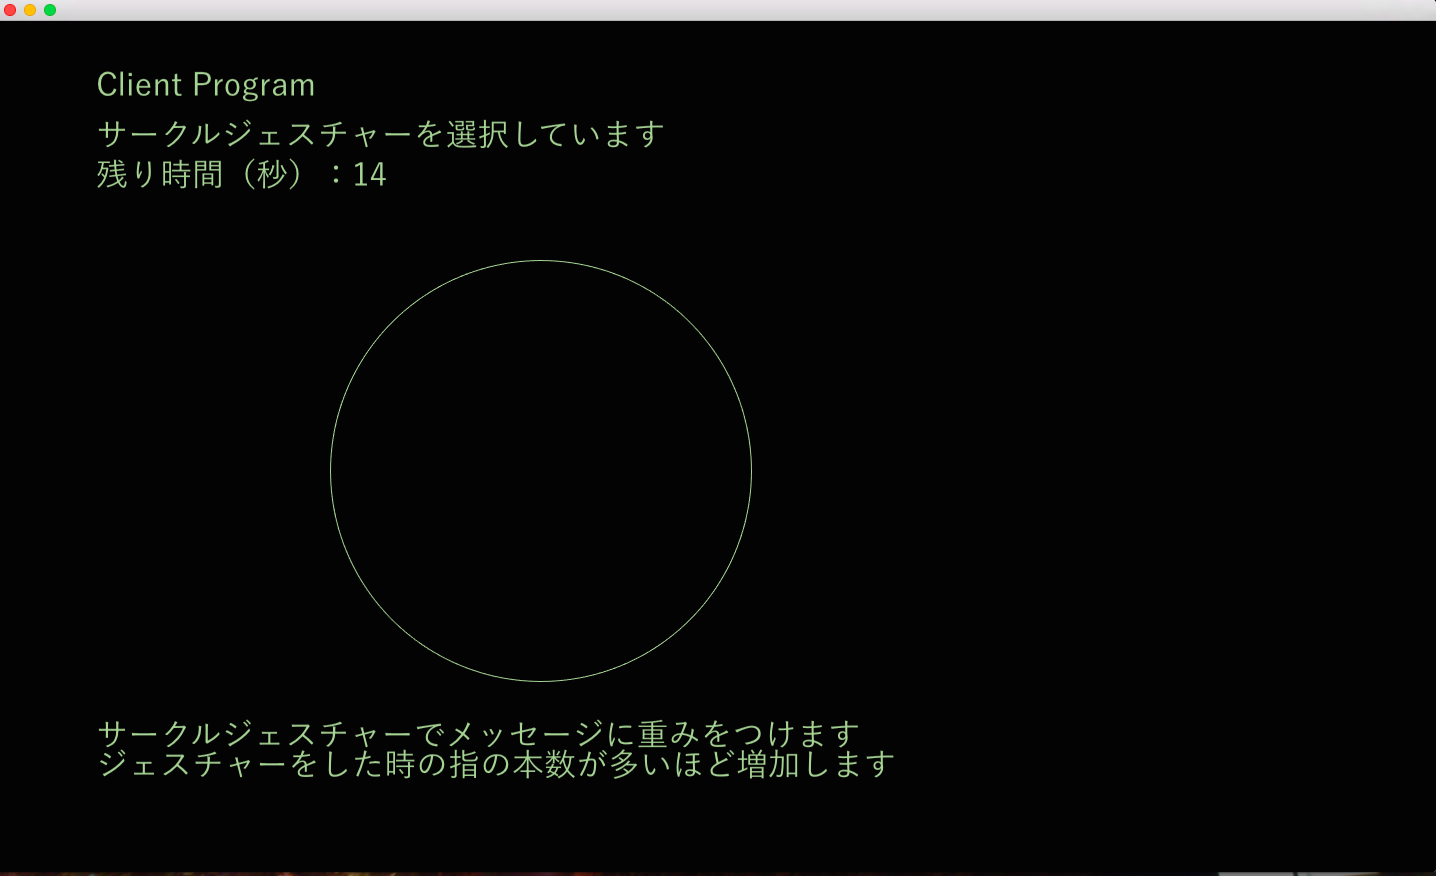
\includegraphics[width=120mm]{./img/clseni3.png}
  \end{center}
  \caption{画面遷移3}
  \label{senni3}
\end{figure}

%どういうメッセージなのか、なぜこのメッセージなのか
%クライアント側からサーバー側のプログラムへ発信される値は以下の5つである. 
%なぜこのような設定になっているのか

\subsubsection{クライアント側から発信する値について}

\begin{itemize}
 \item アカウントナンバー
 \item Leap Morionにかざされている手の数
 \item サークルジェスチャーの回数
 \item スワイプジェスチャーの回数
  \item スクリーンタップジェスチャーの回数
 \item キータップジェスチャーの回数
 \item  メッセージナンバー
\end{itemize}

発信される値は全部で7つある, これらの値は, カンマで区切られた1つの文字列になり, サーバー側へ発信される(図\ref{send}).\\ 
まず, アカウントナンバーはユーザーを特定するための固有な値であり, それぞれの聞き手には予め番号が振り分けられている. これにより誰がどのような値を送ったかを特定しサーバー側で処理する. \\
 次に, 手の数は聞き手がLeap Motionに手をかざしているかの判定に使う. 発信されている値が0の時は, 手をかざしていないことを発信し, 0よりも大きい値の時, 聞き手が手をかざしていることを表す. \\
 各ジェスチャーの回数は, メッセージに重みをつける際に, 聞き手が行ったジェスチャーの回数である. 発信された値は, サーバー側で処理され, 描写に反映される(図\ref{server}参照). 
最後にメッセージナンバーは, 選択したメッセージを表す. 発信するメッセージは9つ用意されており, それぞれ対応した値が発信される. メッセージナンバーは-1と0から8の値で構成されており, -1のときは選択されていないことを表し, 0から8の値ではそれぞれのメッセージ送られる. \\

\subsubsection{Leap Motionで読み取る値と発信するメッセージについて}
Leap Motionで行うことはジェスチャーの判定とジェスチャーのカウントである.  Leap Motionでは, ユーザーが行ったジェスチャーの種類と, ジェスチャーの状態を判定することができる. ジェスチャーの状態とは, ジェスチャーが始まった時, ジェスチャーをしている時, ジェスチャーが終わった時のことを指す. メッセージの選択の際は, 以下の手順で行う. 





\begin{figure}[H]
 \begin{center}
  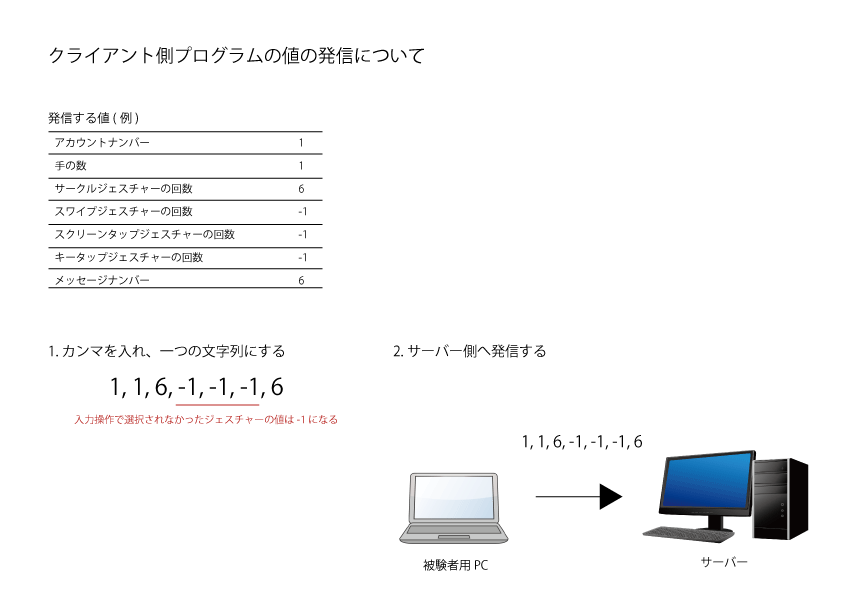
\includegraphics[width=120mm]{./img/sendCL.png}
 \end{center}
 \caption{クライアント側から発信する値}
 \label{send}
\end{figure}

\section{サーバー側のプログラムの役割}
サーバー側プログラムの描写(図\ref{server})はのように行われる. クライアント側プログラムから送られてきた値を集計したものが円の大きさや色で反映される. 以下, それらの役割を記述する. 
 \begin{figure}[H]
 \begin{center}
  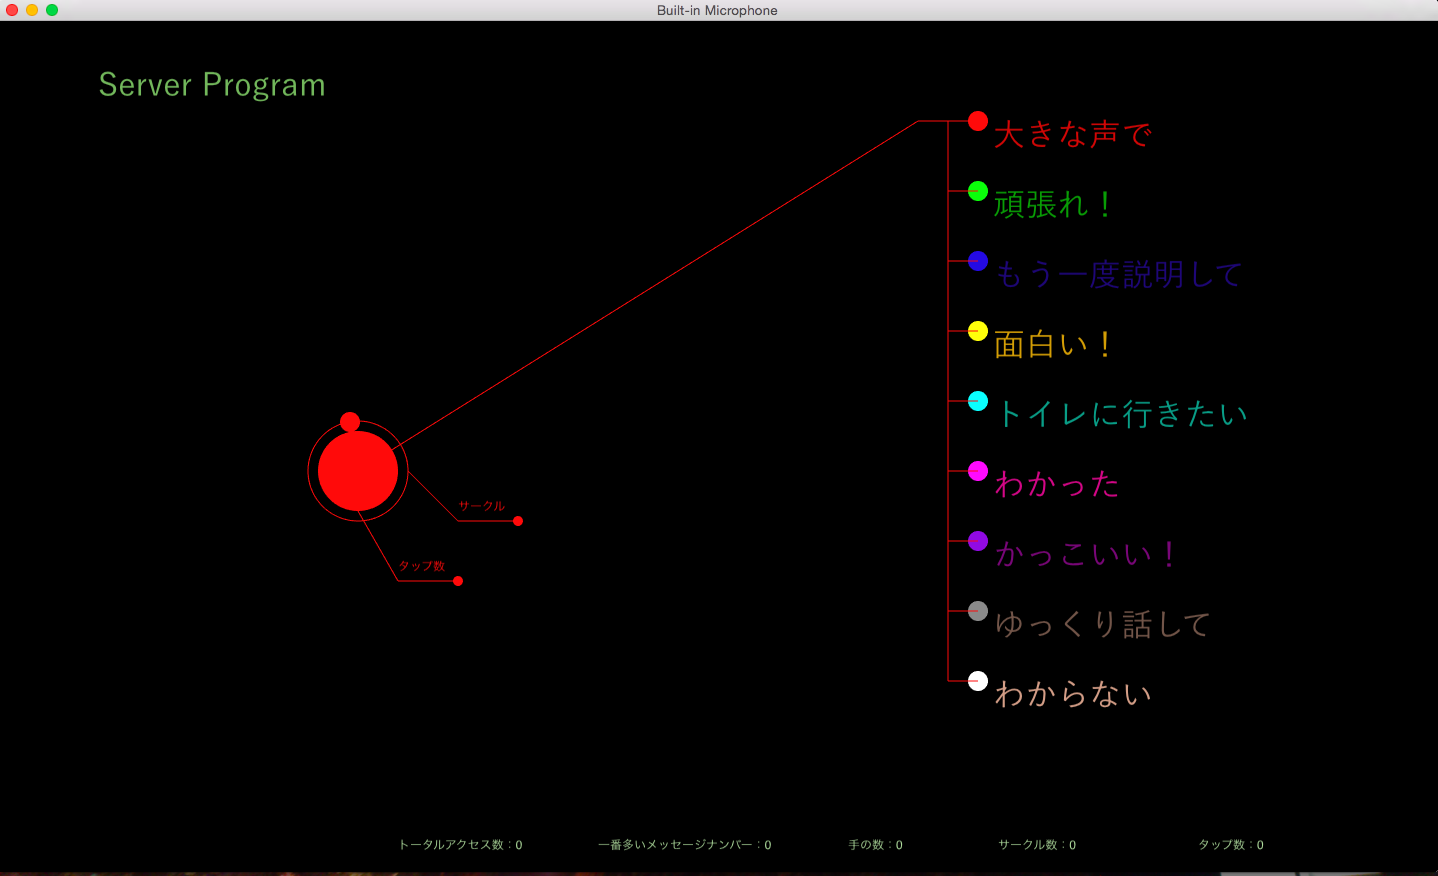
\includegraphics[width=120mm]{./img/server.png}
 \end{center}
 \caption{サーバー側プログラムの描写}
 \label{server}
\end{figure}

\subsubsection{描写処理について}
%どのような描写処理が行われるのか?
図\ref{svcircle}は集計結果を表す円である. 円の色は送られてきたメッセージの多かったものの色に変化する. 変化する色は9つあり, 赤, 緑, 青, 黄, 水色, ピンク, 紫, 灰, 白である. これらの色はメッセージの「大きな声で」から順に対応している(図\ref{svmessage}). 円の直径は発信されたタップするの数によって変化する. クライアント側からメッセージの送信時に送られてきたタップの回数が多いほど, 円は大きくなり, メッセージの重みを示す. 円の外側の小さな円は, 内側の円の円周に沿って回転する. クライアント側からメッセージの送信時に送られてきたサークルジェスチャーの回数が多いほど, 円周を周回する速さが速くなり, メッセージの重みを示す. \\
 また, 図\ref{mario}のマリオネットは図\ref{svcircle}の下面に表示され, 接続されている人数を表す. このシステムは最大で7人が接続されるようになっているので, 最大で7体のマリオネットが表示される. 


\begin{figure}[H]
 \begin{minipage}{0.5\hsize}
  \begin{center}
  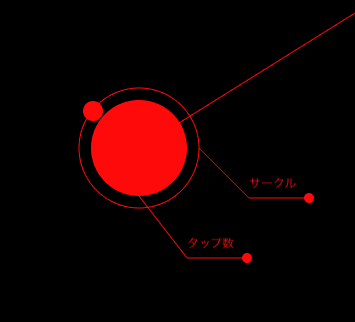
\includegraphics[width=50mm]{./img/svcircle.png}
  \end{center}
  \caption{集計結果を表す円}
  \label{svcircle}
 \end{minipage}
 \begin{minipage}{0.5\hsize}
  \begin{center}
  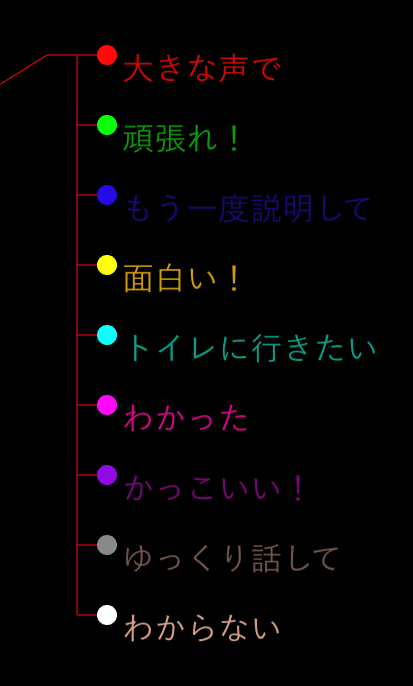
\includegraphics[width=50mm]{./img/svmessagearea.png}
  \end{center}
  \caption{円の色が示すメッセージ}
  \label{svmessage}
  \end{minipage}
\end{figure}

\begin{figure}[H]
 \begin{center}
  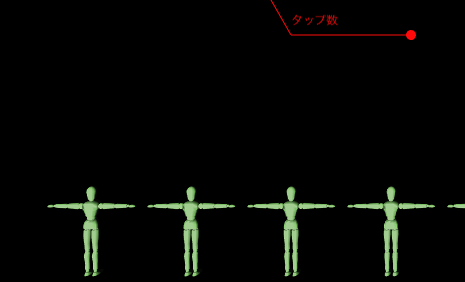
\includegraphics[width=100mm]{./img/mario2.png}
 \end{center}
 \caption{接続されている人数を示すマリオネット}
 \label{mario}
\end{figure}


\subsubsection{メッセージナンバーの集計}
サーバー側では, 聞き手のメッセージを集計し,  その集計結果を発信するためのものである.
まず, 送られてきたメッセージを区切りで分解する. その値を保存する.
送られてきたメッセージは保存後, どのメッセージが多く発信されたかを算出する. 発信されてくるメッセージナンバーは-1から8の値であり, -1のときは代入されない. これにより聞き手が発信した最新のメッセージナンバーが保存される. 一番多く受け取ったメッセージナンバーを算出後, その値にあった描写処理を行う.  

\section{実装方法}

\subsection{言語・ツール・開発環境}
使用言語は主にC++である. 一部, C言語での記述もある. IDEはXcodeでLeap Motionを入力装置として使う. また開発環境は表 \ref{env} の通りである. 

\begin{table}[H]
\begin{center}
\caption{開発環境}
  \begin{tabular}{ll}
  
   \hline
OS & OS X  Yosemite Macbook Air \\ 
  \hline
プロセッサ & 1.6 GHz Intel Core i5\\ 
  \hline
メモリ & 4GB 1600 MHz DDR3\\ 
  \hline
  \end{tabular}
  \label{env}
  \end{center}
\end{table}


\subsection{Cinderフレームワークについて}
CinderはC++で書かれたのフレームワークである. 画像や動画, 音声処理に長けており, ライブラリが用意されている. 今回は, Cinderを使っての導入事例が多くなってきていることから, Cinderを使って開発を進めることにした. 



\subsubsection{openFrameworksとの違い}
%openFrameworksは創造的なコーディングのためのC++のオープンソースツールキットです
ここではopenFrameworks[]について述べる. openFrameworksはC++のオープンソースツールキットである. openFrameworksは, Cinderと同様に、描写処理等に長けたフレームワークでもあり, Leap Motionを使ったアプリケーションで使われるフレームワークとして、この2つが使われていることが多い. 
openFrameworksはCinderよりも歴史がある. openFrameworksは2004年に開発され広まっていったのに対し. Cinderは2010年から広まった. goolgeトレンド(図\ref{API})では, 近年, Cinderの方がopenFrameworksよりも広く利用されてきていることがわかる. 

\begin{figure}[H]
 \begin{center}
  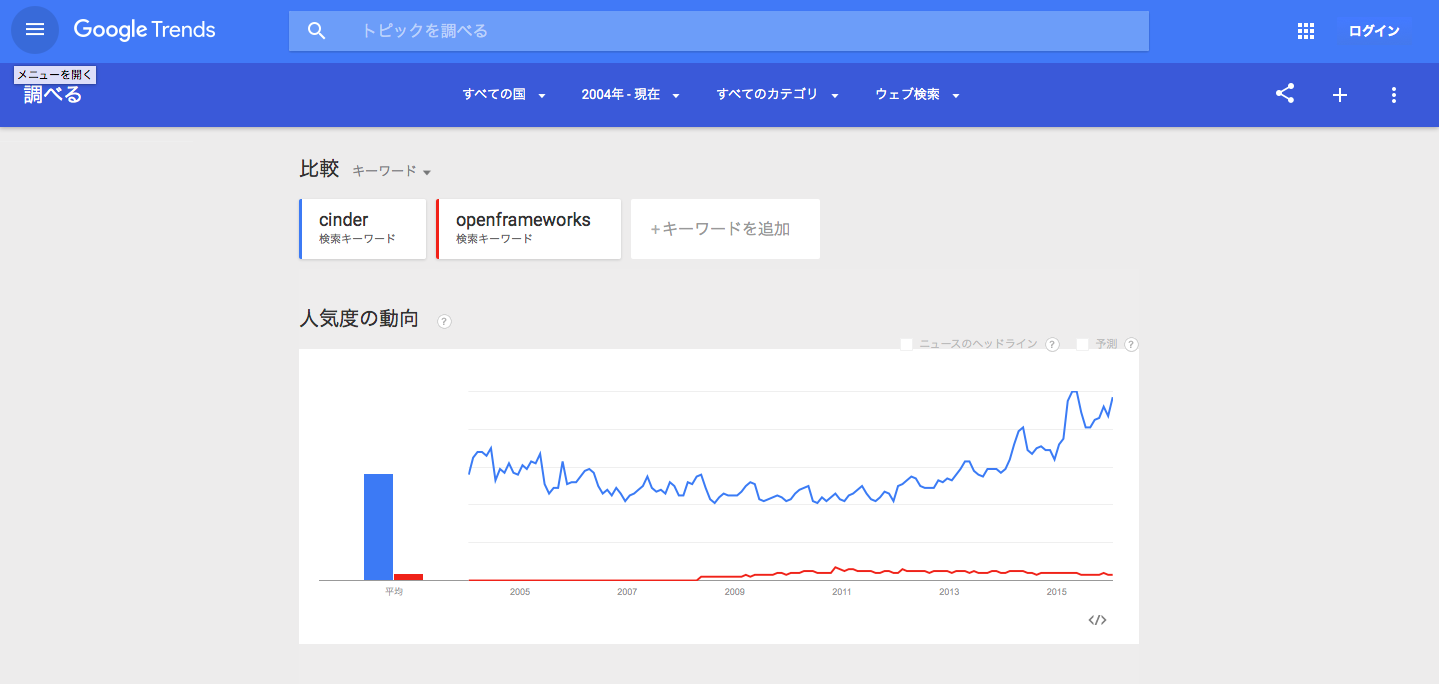
\includegraphics[width=100mm]{./img/api.png}
 \end{center}
 \caption{CidnerとopenFrameworks}
 \label{API}
\end{figure}


\subsection{Leap Motionについて}
%Leap Motionの開発元・リリース時期等を記述.開発言語は
%もっと簡単で良い
Leap Motion(図 \ref{LeapMotion} )とはアメリカのLeap Motion社が2013年にリリースした手や指を検知することに特化したセンサである. Leap Motionは教育に対応するものや医療など幅広く使われている. 開発の可能な言語としては, JavaやC++などの6つが用意されている(図 \ref{Leapdoc}参照).



\begin{figure}[H]
 \begin{center}
  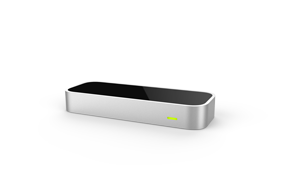
\includegraphics[width=80mm]{./img/LeapMotion.png}
 \end{center}
 \caption{Leap Motion}
 \label{LeapMotion}
\end{figure}

\begin{figure}[H]
 \begin{center}
  
\includegraphics[width=100mm]{./img/Leapdoc.png}
 \end{center}
 \caption{開発の可能な言語}
 \label{Leapdoc}
\end{figure}
この節のLeap Motionに関する画像はLeap Motion SDK から引用.


\subsubsection{Leap Motionの評価}
%Leap Motionの評価
Leap Motionの入力装置としての特性を追求した. ここではLeap Motionの良い点と欠点をあげる. Leap Motionの良い点は, 3つある. \\ 
 1つ目は, Leap Motionでは手や指の位置や方向, ジェスチャーなどを検知し, リアルタイムで入力操作ができるという点である. ジェスチャーは4種類あり, 以下に示す. 先にも述べたが今回のアプリケーションではサークルジェスチャーとスクリーンタップジェスチャーの2種類を検知する. \\

\begin{itemize}
\setlength{\itemsep}{-0.5mm} % 項目の隙間
  \setlength{\parskip}{-0.5mm} % 段落の隙間
 \item サークルジェスチャー:スクリーンに向かって円を描くジェスチャー(図 \ref{circle})
 \item スクリーンタップジェスチャー:スクリーンに向かってタップするジェスチャー(図 \ref{sctap})
 \item スワイプジェスチャー:スクリーン方向にスワイプするジェスチャー(図 \ref{swipe})
 \item キータップジェスチャー:Leap Motion方向にタップするジェスチャー(図 \ref{keytap})
\end{itemize}

\begin{figure}[H]
 \begin{minipage}{0.5\hsize}
  \begin{center}
  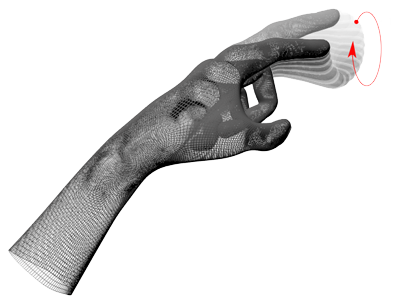
\includegraphics[width=50mm]{./img/Circle.png}
  \end{center}
  \caption{サークルジェスチャー}
  \label{circle}
 \end{minipage}
 \begin{minipage}{0.5\hsize}
  \begin{center}
  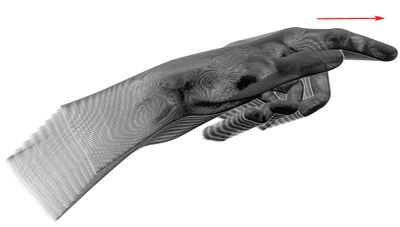
\includegraphics[width=50mm]{./img/ScTap.png}
  \end{center}
  \caption{スクリーンタップジェスチャー}
  \label{sctap}
  \end{minipage}
\end{figure}

\begin{figure}[H]
 \begin{minipage}{0.5\hsize}
  \begin{center}
  
\includegraphics[width=50mm]{./img/Swipe.png}
  \end{center}
  \caption{スワイプジェスチャー}
  \label{swipe}
 \end{minipage}
 \begin{minipage}{0.5\hsize}
  \begin{center}
  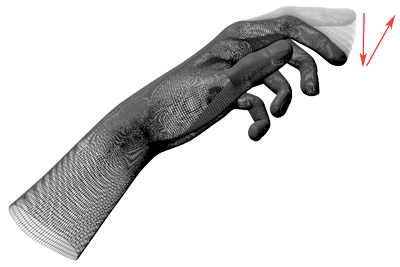
\includegraphics[width=50mm]{./img/KeyTap.png}
  \end{center}
  \caption{キータップジェスチャー}
  \label{keytap}
 \end{minipage}
\end{figure}
%引用元を記述(SDKでいい)
この節のLeap Motionに関する画像はLeap Motion SDK から引用.\\
 
  2つ目は, 指の曲げを判定できるので, 入力パターンが豊富であることがいえる. Leap Motionはどの指が曲げられているか, 曲げられている本数は何本か, どのくらい曲げられているか判定することができる. また, 右手と左手の判定もできるので, 以上のことを使えば入力パターンを増やすことが可能である. \\
   3つ目は, Leap Motionをキーボードやマウスなどの入力装置と比較したとき, 音を出さずに入力できるという利点がある. キーボードやマウスにはボタンがあり, 押すとカチッと音がなる. しかし, Leap Motionは指の曲げやジェスチャー等が入力操作として扱われるので音が出ることはない. \\ 
  一方で, Leap Motionの欠点として次の2つのことを述べる.\\ 
   1つ目は, 特定の方向ではセンシングが難しいことである. Leap Motionは赤外線センサーで感知しており,  図\ref{leap}のような逆四角錐の範囲で検知される. そのため手を地と垂直に向けると手のひらで指を隠してしまうため, 誤検知される危険性がある. よって, 意識して地と平行にかざすことでLeap Motionが誤操作が発生しにくいことがわかった.\\
   もう1つは, 複数接続が不可能であることである. 1台のPCに接続できるのは1つのLeap Motionで, 2つ以上繋いだ場合, 1台目のLeap Motionが優先され, 2台目は機能しないことがわかった.\\ 
 
 \begin{figure}[H]
 \begin{center}
  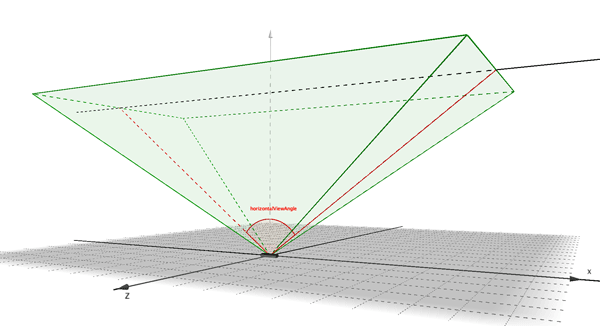
\includegraphics[width=100mm]{./img/LeapAngle.png}
 \end{center}
 \caption{Leap Motionのセンサ範囲}
 \label{leap}
\end{figure}

この節のLeap Motionに関する画像はLeap Motion SDK から引用.

%\subsubsection{ソケット通信について}
%ソケット通信とは。なぜ、どういう意図で通信するのか
%ソケット通信:ソケットというプログラム間でデータの送受信を行うための標準的なプログラムインタフェース(API)を使ってプログラム同士で通信を行うことを指す
%\subsubsection{全体像}


%\begin{figure}[H]
 %\begin{center}
 %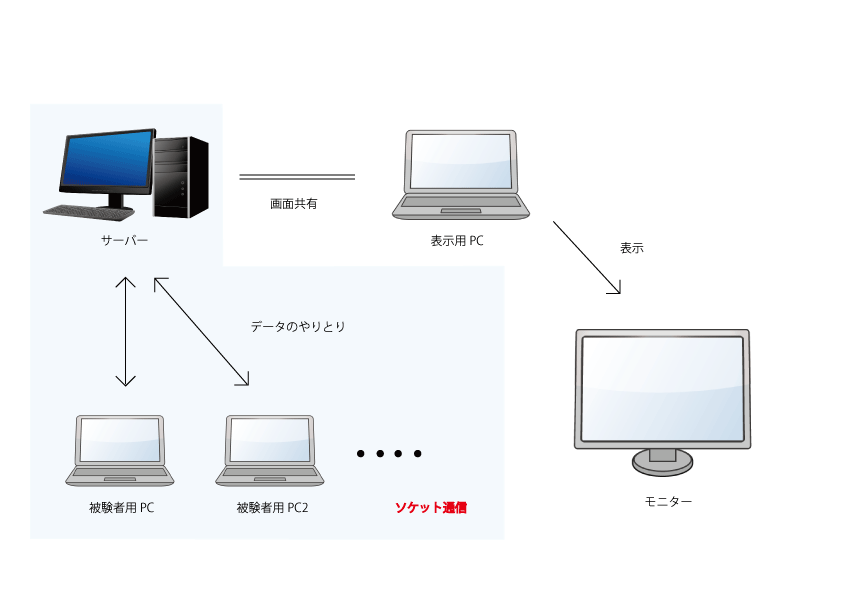
\includegraphics[width=100mm]{./img/zentai.png}
 %\end{center}
% \caption{全体像}
 %\label{zentai}
%\end{figure}

%--------------------------------------------------------------------
%全体を通して(1/12)
%受講者は発表者に何が伝えられるのか。通信することによって何がおこるのか。何を起こしたいのかについて詳しく述べるべき。

%--------------------------------------------------------------------
\chapter{実験と評価}

\section{実験の目的}
本実験ではゼミを行っている間に自然なかたちで話し手に情報を伝達できるようにする. 例えば,  聞き手側が話し手の話すスピードが速いと思ったとする. このとき聞き手側に本システムを使用してもらい, 「話すスピードが速い」とメッセージの発信を行う. このような状況下で, 提案するシステムが話し手にどのようなリアクションを起こすのか, 話し手の邪魔になっていないかどうかを調査するために行った. 

\section{方法}
\subsection{日時と場所}

本実験は1月27日, 公立はこだて未来大学の1Fスタジオの教員室132前で行った. 
 \begin{figure}[H]
 \begin{center}
  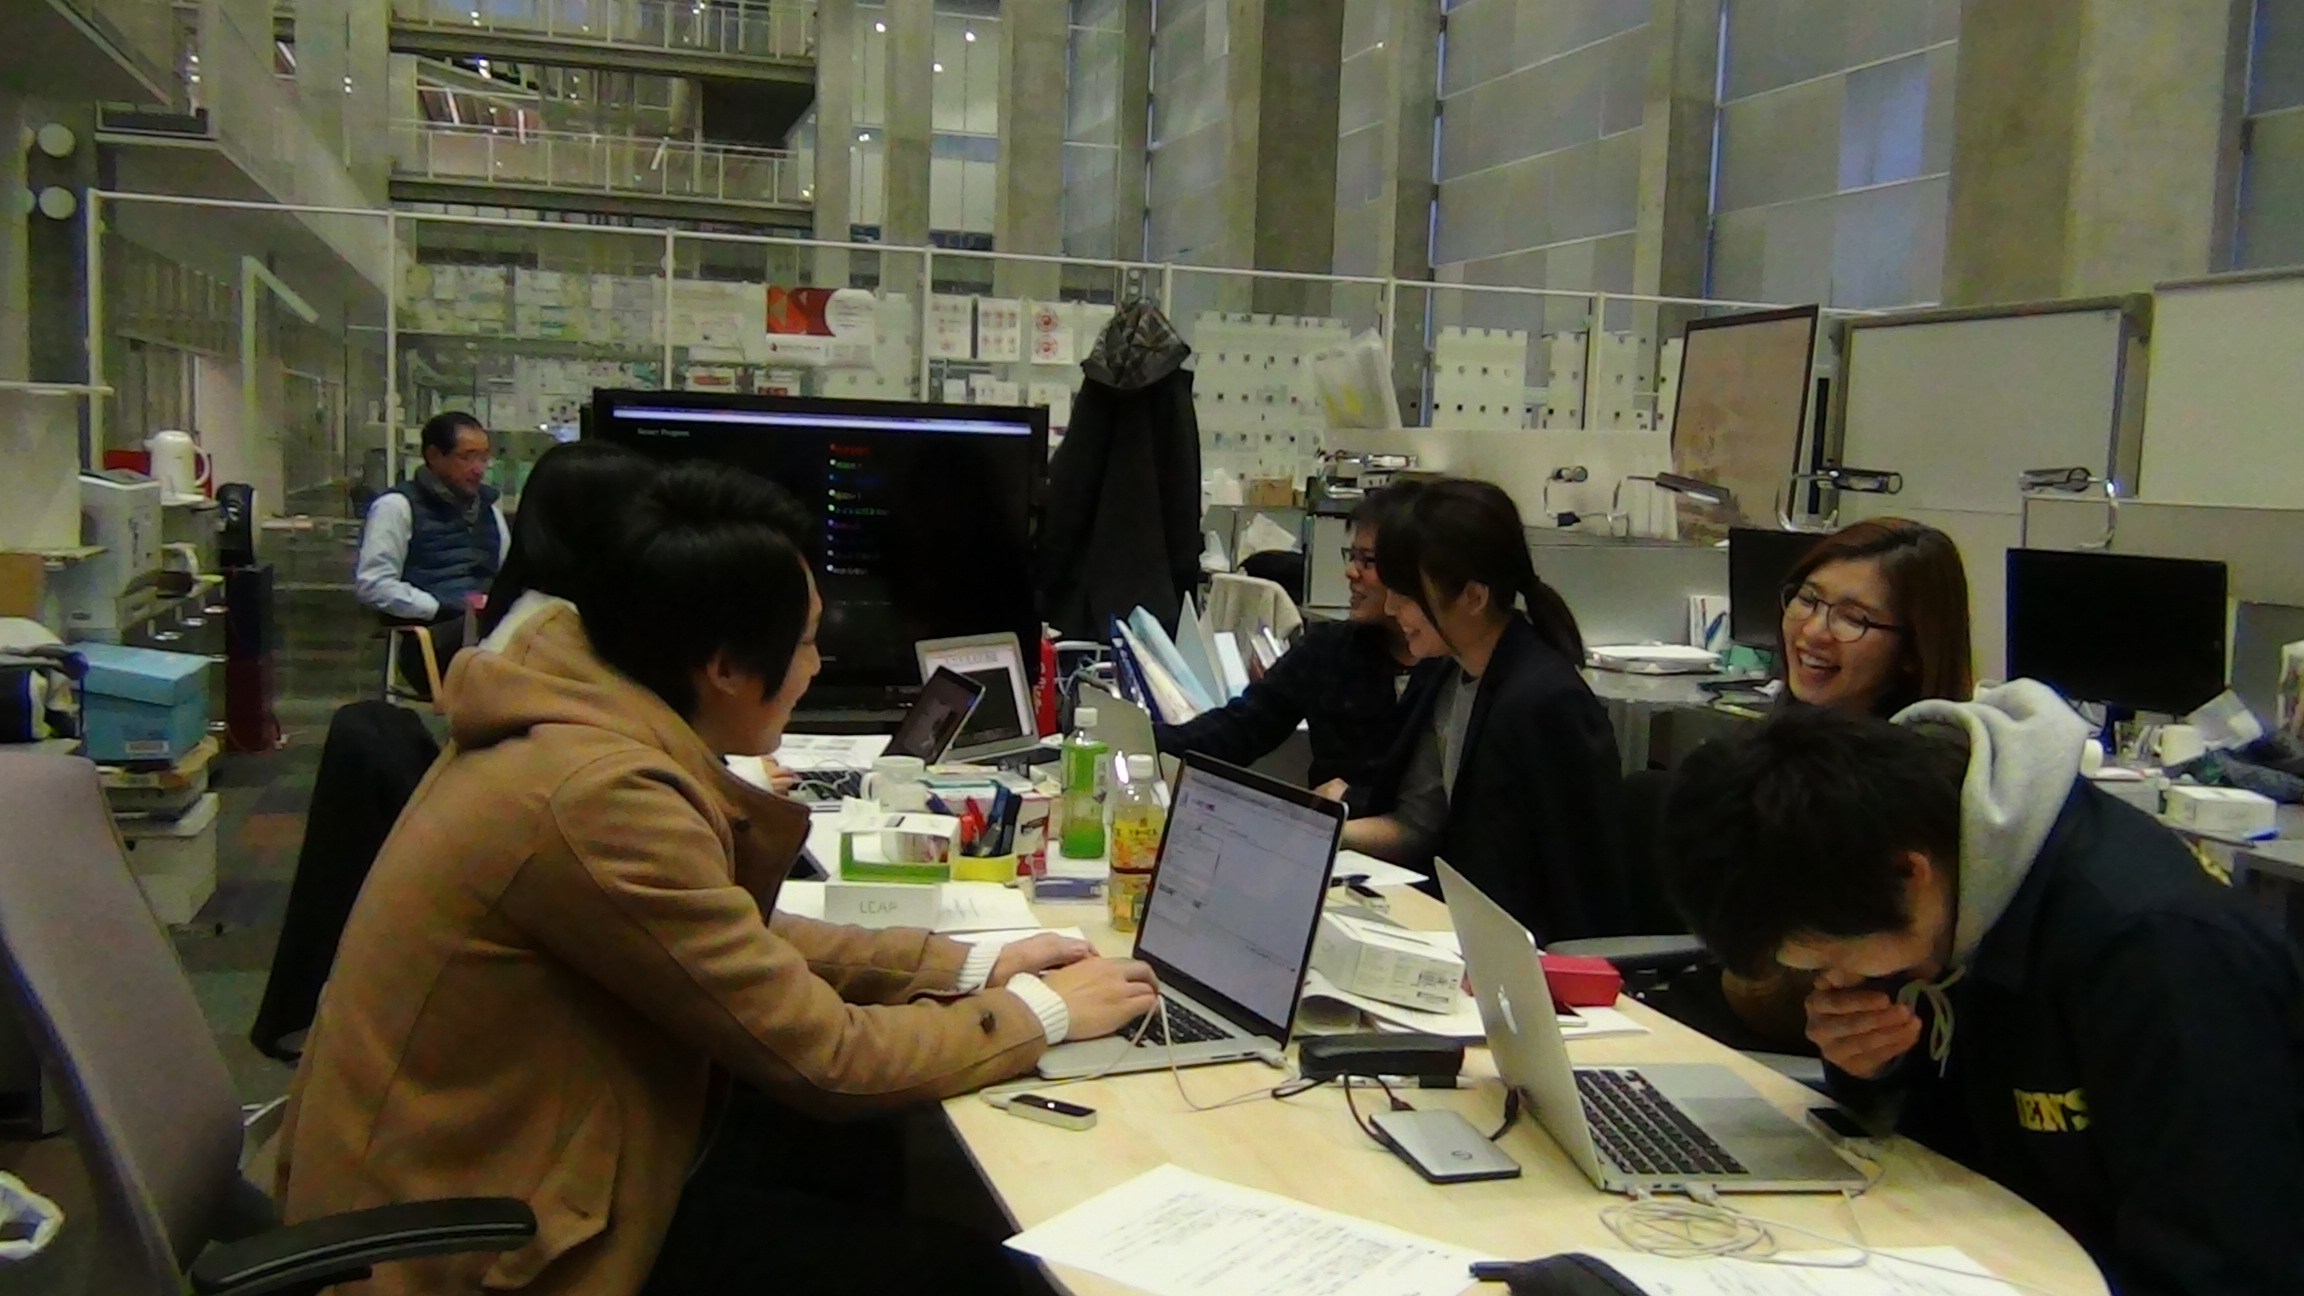
\includegraphics[width=120mm]{./img/DSC00031.JPG}
 \end{center}
 \caption{実験の様子}
 \label{zi}
\end{figure}

\subsection{被験者}
被験者は公立はこだて未来大学の大学生6人で, 男性が3人, 女性が3人である. 

\subsection{道具}
本実験で使用した道具は表\ref{tools}のとおりである. 

\begin{table}[H]
\begin{center}
\caption{実験器具}
  \begin{tabular}{ll}
   \hline
   道具名 & 台数\\
   \hline
   Macbook & 6台\\
   \hline
   Leap Motion & 6台\\ 
   \hline
  ビデオカメラ & 1台\\ 
   \hline
   \end{tabular}
   \label{tools}
  \end{center}
\end{table}


\subsection{手順}
本実験を行うにあたり, 以下の手順で行うことを被験者に説明した.  

\begin{enumerate}
\renewcommand{\labelenumi}{\arabic{enumi}}
 \item Leap Motionが使用できることを確認する(付録2参照).
 \item visualiserで一度手が検知されていることを確認する(付録2参照).
 \item 被験者は話し手と聞き手に分かれる. 
 \item 実験者は被験者全員にクライアント側のプログラムを配布する.
 \item 実験者はサーバー側のプログラムを起動する. 
 \item 聞き手ははゼミが始まると同時にプログラムを起動する. 
 \item 両方のプログラムの起動を確認後, 話し手が進捗報告を行う. 
 \item 被験者には伝えたいメッセージがあるときにアプリケーションを使って発信してもらう.
 \item 話し手の進捗報告が終わると, 聞き手は話し手に質問やコメントを述べる.
 \item 被験者はアンケートに回答する.
\end{enumerate}

\subsection{アンケート}
アンケートは5段階評価の質問を8つと自由記述を2つ設けた. \\
\subsubsection{5段階評価の質問}
\begin{enumerate}
\renewcommand{\labelenumi}{\arabic{enumi}}
 \item 自分のメッセージが発信されたことについてわかりやすかったと思う
 \item サーバー側プログラムの変化がわかった
 \item 表示されているものの役割・意味についてまで理解することができたと思う(クライアント側) 
 \item 表示されているものの役割・意味についてまで理解することができたと思う(サーバー側)
 \item 話し手の進捗報告は十分に理解できたと思う 
 \item メッセージの発信後, またはサーバー側プログラムの表示の変化後, 話し手にリアクションがあったと思う
 \item アプリケーションは話し手の邪魔をしていたと思う
 \item メッセージの候補の数は適当だと思う
\end{enumerate}
\subsubsection{自由記述}
\renewcommand{\labelenumi}{\arabic{enumi}}
\begin{enumerate}
 \item 他にも話し手に伝えたいメッセージがあれば教えてください
 \item 意見や感想, アドバイスなど
\end{enumerate}


\subsection{アンケート結果}
ここではアンケートの集計結果と自由記述で書かれていたことを記す. 

\subsubsection{アンケート集計結果}
\begin{figure}[H]
 \begin{minipage}{0.5\hsize}
  \begin{center}
  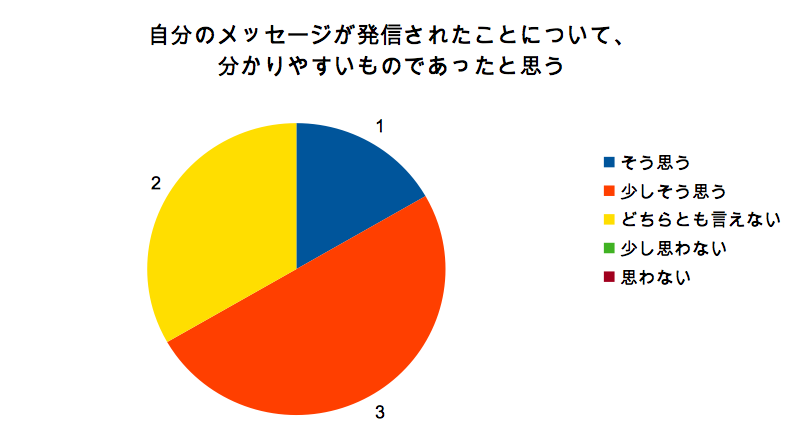
\includegraphics[width=70mm]{./img/question1.png}
  \end{center}
  \caption{自分のメッセージが発信されたこと\newline についてわかりやすかったと思う}
  \label{question1}
 \end{minipage}
 \begin{minipage}{0.5\hsize}
  \begin{center}
  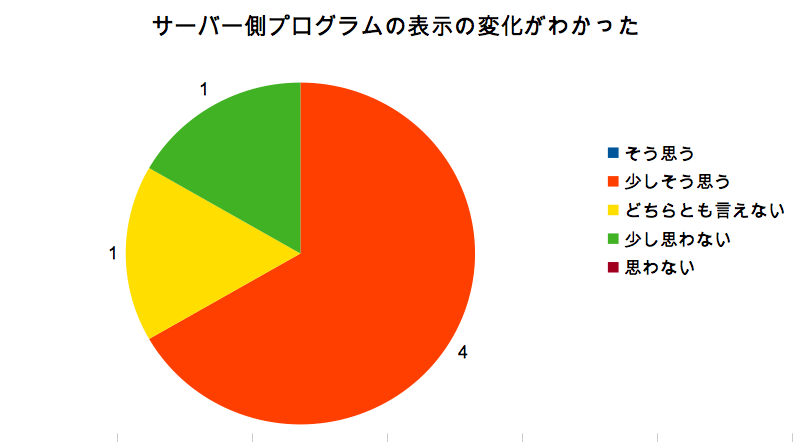
\includegraphics[width=70mm]{./img/question2.png}
  \end{center}
  \caption{サーバー側プログラムの変化\newline がわかった}
  \label{question2}
  \end{minipage}
  \end{figure}

\begin{figure}[H]
 \begin{minipage}{0.5\hsize}
  \begin{center}
  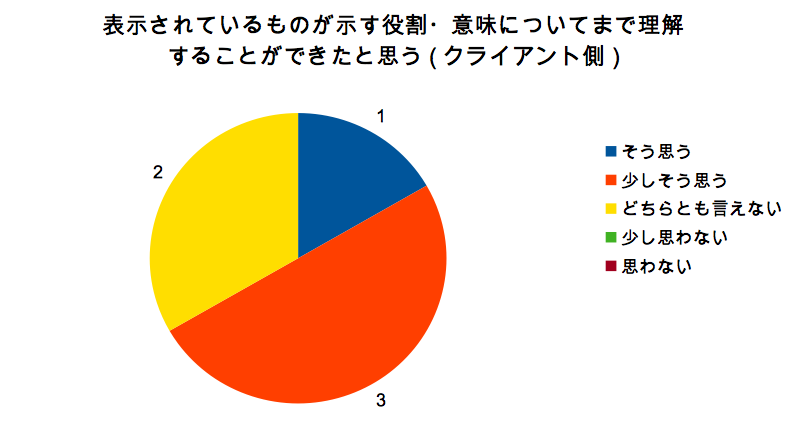
\includegraphics[width=70mm]{./img/question3.png}
  \end{center}
  \caption{表示されているものの役割・意味\newline についてまで理解することができた\newline と思う(クライアント側)}
  \label{question3}
 \end{minipage}
 \begin{minipage}{0.5\hsize}
  \begin{center}
  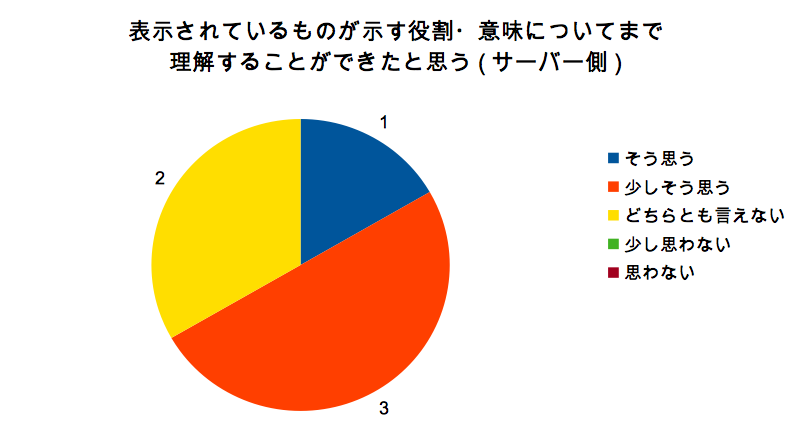
\includegraphics[width=70mm]{./img/question4.png}
  \end{center}
  \caption{表示されているものの役割・意味\newline についてまで理解することができた\newline と思う(サーバー側)}
  \label{question4}
  \end{minipage}
  \end{figure}
  
  \begin{figure}[H]
 \begin{minipage}{0.5\hsize}
  \begin{center}
  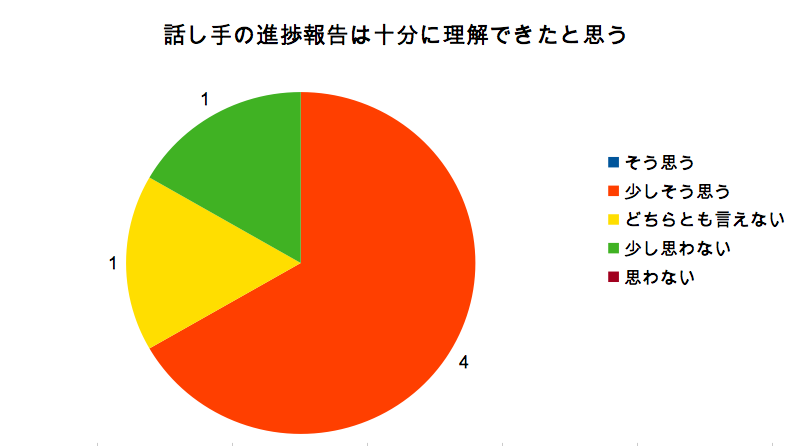
\includegraphics[width=70mm]{./img/question5.png}
  \end{center}
  \caption{話し手の進捗報告は十分に聞けた\newline と思う}
  \label{question5}
 \end{minipage}
 \begin{minipage}{0.5\hsize}
  \begin{center}
  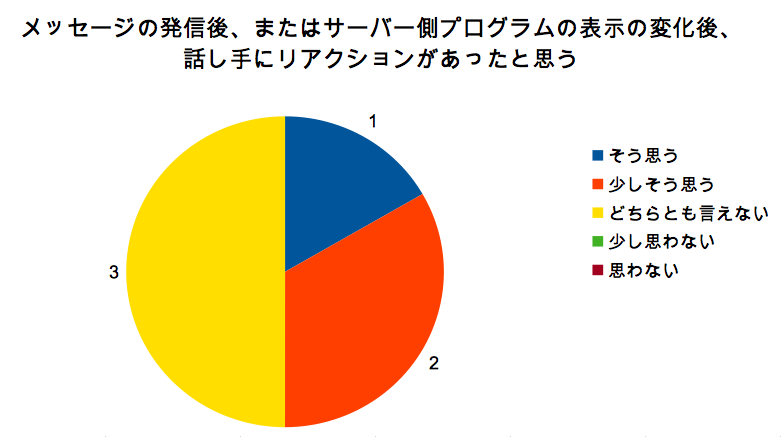
\includegraphics[width=70mm]{./img/question6.png}
  \end{center}
  \caption{メッセージの発信後, またはサーバー側プログラムの表示の変化後, 話し手に\newline リアクションがあったと思う}
  \label{question6}
  \end{minipage}
  \end{figure}
  
  \begin{figure}[H]
 \begin{minipage}{0.5\hsize}
  \begin{center}
  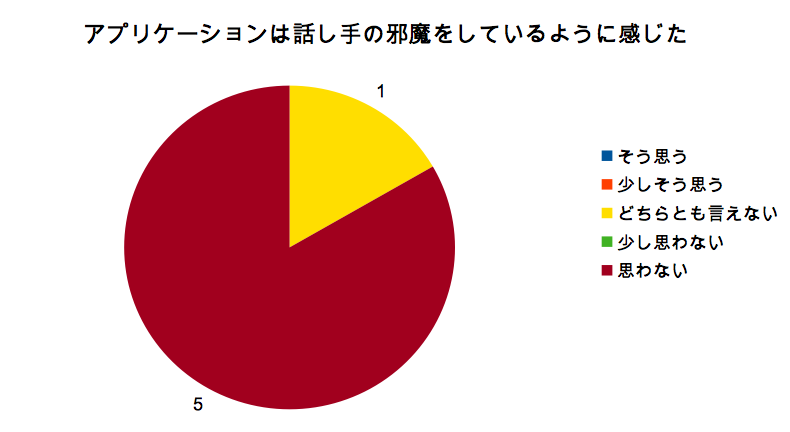
\includegraphics[width=70mm]{./img/question7.png}
  \end{center}
  \caption{アプリケーションは話し手の邪魔\newline をしているように感じた}
  \label{question7}
 \end{minipage}
 \begin{minipage}{0.5\hsize}
  \begin{center}
  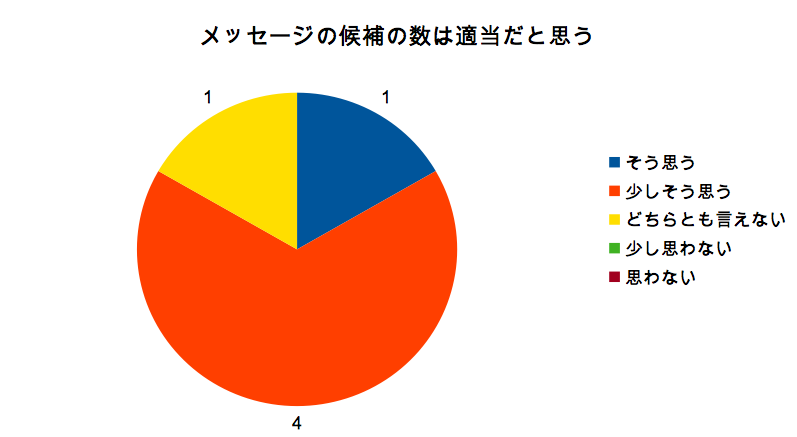
\includegraphics[width=70mm]{./img/question8.png}
  \end{center}
  \caption{メッセージの候補の数は適当だったと思う}
  \label{question8}
  \end{minipage}
  \end{figure}

図\ref{question1} より, 自分のメッセージが発信されたことについてわかりやすかったと思うという問いに対して, 4名が思うという方に回答をし, 2名がどちらとも言えないと答えた. これに関しては, 発信されたメッセージが話し手にしか見るようにしていなかったためだと考えられる. \\

図\ref{question2} より, サーバー側プログラムの変化がわかったという問いに対して, 4名がわかったという方に回答をし, 1名の人がどちらとも言えない, 1名がわからなかったと答えた. このわからなかったという1名に関しては, 円の大きさや周りを沿って移動する円のスピードの変化がわかりにくかったと考えられる. \\ 

図\ref{question3} より, 表示されているものの役割・意味についてまで理解することができたと思う(クライアント側)という問いに対して, 4名の人が思うという方に回答をし, 2名の人がどちらとも言えないと答えた. \\

図\ref{question4} より, 表示されているものの役割・意味についてまで理解することができたと思う(サーバー側)という問いに対して, 4名の人が思うという方に回答をし, 2名の人がどちらとも言えないと答えた. \\

図\ref{question5} より, 話し手の進捗報告は十分に理解できたと思うという問いに対して, 4名の人が思うという方に回答をし, 2名の人がどちらとも言えないと答えた. これに関しては, Leap Motionを操作することに注意が向き, 話を聞けなかったことが考えられる. また「もう一度説明してください」のメッセージを発信しても話し手からのリアクションが得られなかった可能性がある. \\

図\ref{question6} より, メッセージの発信後, またはサーバー側プログラムの表示の変化後, 話し手にリアクションがあったと思うという問いに対して, 3名の人が思うという方に回答をし, 3名の人がどちらとも言えないと答えた. この結果から, 話し手のリアクションはあったということがいえる. ただし, 話し手が全てのメッセージに気づき, 応答できなかった可能性が考えられ, そのため3名がどちらともいえないという回答になったとかんがえられる. \\

図\ref{question7} より, アプリケーションは話し手の邪魔をしていたと思うという問いに対して, 5名の人がそう思わないという方に回答をし, 1名の人がどちらとも言えないと答えた. このことから本システムは話し手の邪魔にならなかったということがいえる. \\

図\ref{question8} より, メッセージの候補の数は適当だと思うという問いに対して, 5の人が思うという方に回答をし, 1名の人がどちらとも言えないと答えた. この結果から, メッセージの候補数は概ね適当であったということがいえる. \\

\subsubsection{自由記述の結果}
他にも話し手に伝えたいメッセージがあれば教えてください\\

\begin{itemize}
\setlength{\itemsep}{-0.5mm} % 項目の隙間
  \setlength{\parskip}{-0.5mm} % 段落の隙間
%\renewcommand{\labelenumi}{\arabic{enumi}}
 \item 講義などのシーンに関しては現状で良いと思います.\\
 \item スライドが見易い.\\
 \item 話すスピードが速い.\\
 \item 伝えたいものというより、30秒待たないと発信できないもどかしさがあった。メッセージの種類は丁度良かったと思う.\\
 \item メッセージの種類は丁度良いと思います.\\
 \item おなかがすいたとか休憩したいとか送りたかった.\\
 \item トイレに行きたい、おなかがすいたなどを全部まとめて「休憩したい」にしても良いように感じた.\\
\end{itemize}

意見や感想, アドバイスなど\\
\begin{itemize}
\setlength{\itemsep}{-0.5mm} % 項目の隙間
  \setlength{\parskip}{-0.5mm} % 段落の隙間
%\renewcommand{\labelenumi}{\arabic{enumi}}
 \item メッセージ選択までの時間が30秒だと少し長いように感じました.\\
 \item 前回と比較して、メッセージを決定するまでの動作が簡単になったため、もう少し選択時間が短くても良いのかな、と感じました. でも、選択した瞬間にサーバー側にすぐに行っているみたいなので、その点はリアルタイムなコメントがもらえて良いと思いました.\\
 \item 2つ目の画面の円の大きさを送る場面は, 時間が長すぎる. 15秒くらいでいいと思う.\\
 \item 入力画面の時間制限を目立つ形で表示すると、誤送信を防げると思う.\\
 \item かっこいいがくると、とても嬉しかった. 色でメッセージが判断できるのは, わかりやすくて良いと思います.\\
 \item 真ん中の円の視認性をあげた方がいい. 発表者は自分の発表に集中しながらその画面を見るわけだから, 視野に入った時点で, 聞き手が何を合図したかわかるように円を大きくしたり工夫をするといいかも.\\
% \item 複数人で使用できたり, すぐにメッセージを送る事ができた方がよかったと思いました\\
 \item 私のPCがみんなと画面サイズが異なるせいか, 下のメッセージ(小さく書いていた文字)が全て見えなかった. そのため, なにが送られたか謎だった. \\
 \item 選択したメッセージを取り消す方法がわからなかった. 
 \item サーバー画面(話し手が見るべき画面)の置き場によって, 結果が変わってしまうように感じた. 話し手と話し手が使うモニターの間にサーバー画面を置いた方がもっとこのツールの良さが出てくると感じた. サーバー画面は話し手だけではなくゼミ生みんなに見えてもおもしろいかも!\\
 \item わかったとかっこいいの色の区別がしにくかった.\\
 \item 以前よりも格段に操作がしやすかった\\これをゼミ生みんなで使えたらゼミがもっと充実したものになると思う\\
 \item 自分の意思で「送信」できないのは「自分のメッセージが発信されたことについて、分かりやすいもの」かと考えたときに分かりづらいと思う.\\
 \item あと,  時間制限があるためメッセージの選択権利と重要性が自分の意思と反して伝わってしまう場合が多いと感じられた\\
 \item 話し手が見る画面. Helpが欲しい\\
 \item UIはシンプルでいいと思う.逆に伝わりづらくなってる部分もある. (例えば, サーバー画面で発信されたメッセージは色でわかりやすいがメッセージの重さがシステムを知らない人からしたら味方がわかりにくいと感じた.)\\
\end{itemize}






%\subsection{初心者}

%Java言語との比較では,惨敗であり,FUNは2倍の記述量を必要とした.しかし,これは,JavaのもつパッケージIKURAが非常に強力であるためで,同一機能をもつライブラリを用意することにより,FUNにも同様の能力を持たせることができることが判明した.

%\subsection{上級者}

%Java言語との比較では,惨敗であり,FUNは2倍の記述量を必要とした.しかし,これは,JavaのもつパッケージIKURAが非常に強力であるためで,同一機能をもつライブラリを用意することにより,FUNにも同様の能力を持たせることができることが判明した.

%--------------------------------------------------------------------
\chapter{考察}
\section{話し手のシステムに対するリアクション}
本実験のアンケート結果から, 話し手のアプリケーションに対するリアクションは半数の人があったと答え, 半数がどちらともいえないということがわかった. この結果に関して, 実際の実験の様子から, 話し手がアプリケーションを見るのは説明しているスライドや聞き手の顔を見る時間と比べて極めて少ない時間であり, 送られてきたメッセージ全てを確認できなかったのではないかと考えられる. また, 発信されてきたメッセージに気付けても, 瞬時に対応するのが難しかったとも考えられる. これらに関しては話し手が見るサーバー側プログラムの位置を変えたり, 大きなモニター等に表示することで, 話し手が変化に気づき, 対応できると考えられる. その他にも描写の色や大きさが変化した時に, 色やアニメーション等のエフェクトを入れることで話し手が変化に気づきやすくなると考えられる. 自由記述の部分では, かっこいいなどの話し手を賞賛するメッセージが発信された時, 話し手が嬉しくなることがわかった. このように聞き手側から話し手側へメッセージを発信することによって, 今まで話し手が情報を発信するだけだったものが聞き手の想いを汲み取り, リアクションができるように, 相互的な状態が作り出せたと考えられる. 

%Java言語との比較では,惨敗であり,FUNは2倍の記述量を必要とした.しかし,これは,JavaのもつパッケージIKURAが非常に強力であるためで,同一機能をもつライブラリを用意することにより,FUNにも同様の能力を持たせることができることが判明した.

\section{話し手の邪魔になっていないか}
本実験のアンケート結果から, 話し手の邪魔になっていないかという問いに対して, 5名が思わないと答え, 1名がどちらとも言えないということがわかった. このことから概ね話し手に与えるストレスは少ないということがいえる. ただ色の判別や文字の大きさなど, 視認性をあげることで話し手がメッセージに気づく可能性が上がるのではないかと考えられる. 

%\section{本システムについて}
%本システムではLeap Motionでジェスチャーを使ってメッセージの発信をおこなった. そのなかでメッセージの発信までの時間の設定という面で改善がみられる. 



%Java言語との比較では,惨敗であり,FUNは2倍の
%記述量を必要とした.しかし,これは,Javaのもつ
%パッケージIKURAが非常に強力であるためで,
%同一機能をもつライブラリを用意することにより,
%FUNにも同様の能力を持たせることができることが判明した.


%--------------------------------------------------------------------
\chapter{結論と今後の展開}

\section{まとめ}
本研究では, 授業中や大学のゼミ中を想定し, 聞き手側からLeap Motionを操作し, 話し手側にメッセージを発信するためのアプリケーションを開発した. これにより, 聞き手が話し手にメッセージを送信することで, 話し手がリアクションを起こし, 対話的な授業運営, ゼミの進行を目指すことを目的とした. 実験結果から聞き手から話し手にメッセージの発信した際, 話し手がリアクションを行うことや, それが話し手にストレスを与えるものではないということがわかった. また, 視認性をあげることやメッセージを発信するまでの時間について課題がみられた. 
%聞き手側から話し手にメッセージを送信することでリアクションを受け取れるのか, 話し手の邪魔になることはないか


%Java言語との比較では,惨敗であり,FUNは2倍の記述量を必要とした.しかし,これは,JavaのもつパッケージIKURAが非常に強力であるためで,同一機能をもつライブラリを用意することにより,FUNにも同様の能力を持たせることができることが判明した.

%Java言語との比較では,惨敗であり,FUNは2倍の記述量を必要とした.しかし,これは,JavaのもつパッケージIKURAが非常に強力であるためで,同一機能をもつライブラリを用意することにより,FUNにも同様の能力を持たせることができることが判明した.

%Java言語との比較では,惨敗であり,FUNは2倍の記述量を必要とした.しかし,これは,JavaのもつパッケージIKURAが非常に強力であるためで,同一機能をもつライブラリを用意することにより,FUNにも同様の能力を持たせることができることが判明した.

\section{今後の方針}
本研究では, 実験の結果から視認性に対して課題があると感じた. 文字の色や大きさなどである. これを改善することで話し手がメッセージに気づく可能性が上がり, 聞き手が発信したメッセージに対して, 話し手からの良いリアクションが得られると考えられる. 

%Java言語との比較では,惨敗であり,FUNは2倍の記述量を必要とした.しかし,これは,JavaのもつパッケージIKURAが非常に強力であるためで,同一機能をもつライブラリを用意することにより,FUNにも同様の能力を持たせることができることが判明した.


%--------------------------------------------------------------------
\chapter*{謝辞}
本研究を進めるにあたり, ご指導いただいた美馬義亮先生に感謝いたします. また, アドバイスやご指摘をしてくれた美馬研究室の学生の皆様, 実験に協力してくださった学生の皆様に感謝申し上げます. 


%--------------------------------------------------------------------
% 参考文献
\begin{thebibliography}{9}
 \bibitem {A1} 学制百年史, 明治初期の高等教育, \url{http://www.mext.go.jp/b_menu/hakusho/html/others/detail/1317598.htm},2015
   \bibitem {A2} 武田直人 田口忠緒,  クリッカー(授業応答システム)を用いた双方向性授業の比較と評価:学生中心学習の構築を目指して, 名城大学薬学部薬学教育開発センター, \url{http://www.keepad.com/jp/casestudies/docs/Comparison%20and%20Evaluation%20of%20Clikers%20in%20the%20Interactive%20Classroom.pdf}, 2012.
 \bibitem {A3} 株式会社サイボウズ, "サイボウズlive", https://live.cybozu.co.jp/overview.html, 参照 2016年1月25日.
  \bibitem {A4} 中村薫, 「Leap Motion プログラミングガイド 改訂版」, 2015.
  \bibitem {A5} クリッカー Socratec Nano Type-T 使用のTIPS, \url{http://www.a.math.ryukoku.ac.jp/~hig/eproj/clicker/tips_nano.php}, 2015年1月28日参照.
% \bibitem {A1} ソケット通信, http://www.linuxhowtos.org/C_C++/socket.htm, 2003.
 %\bibitem {A1} 著者, 「タイトル」, 2003.
\end{thebibliography}





% 以降,付録(付属資料)であることを示す
\appendix

%--------------------------------------------------------------------
\chapter*{付録その1 アンケート} % \chapter{}を使うと「付録A ***」となる

 \begin{figure}[H]
 \begin{center}
  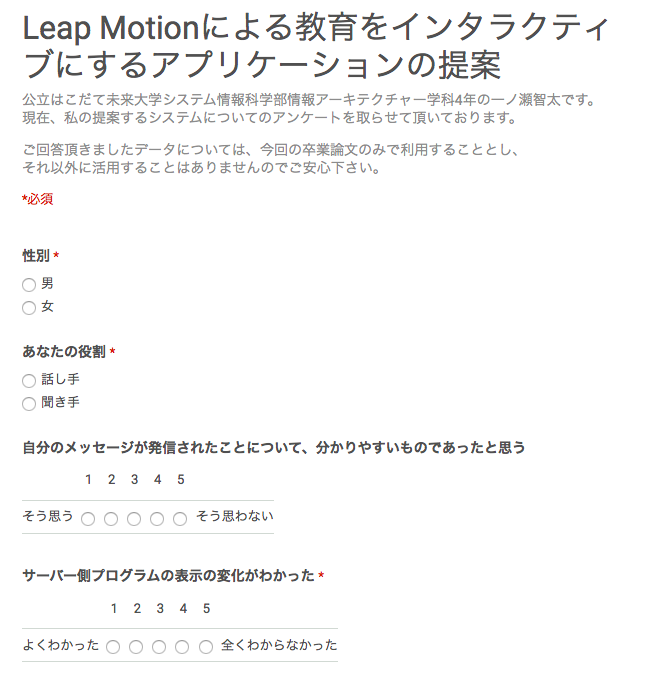
\includegraphics[width=120mm]{./img/ank1.png}
 \end{center}
 \caption{使用したアンケート1}
 \label{leap}
\end{figure}

 \begin{figure}[H]
 \begin{center}
  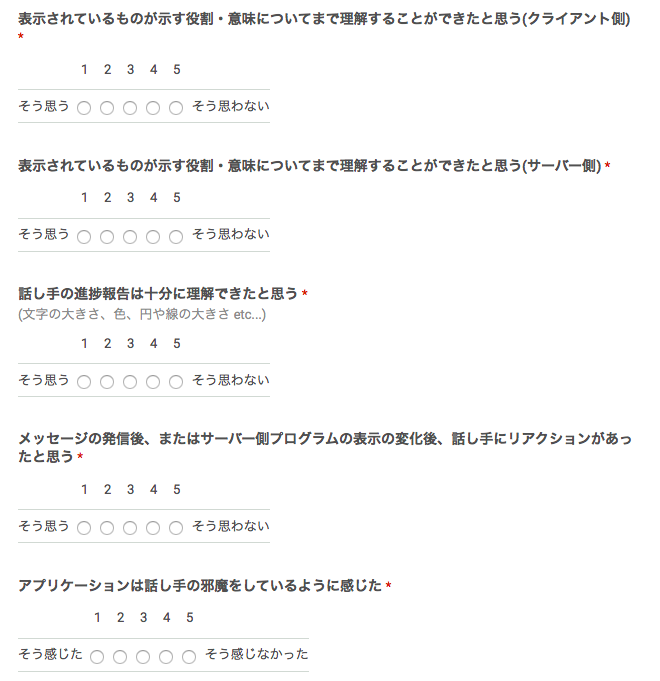
\includegraphics[width=120mm]{./img/ank2.png}
 \end{center}
 \caption{使用したアンケート2}
 \label{leap}
\end{figure}

 \begin{figure}[H]
 \begin{center}
  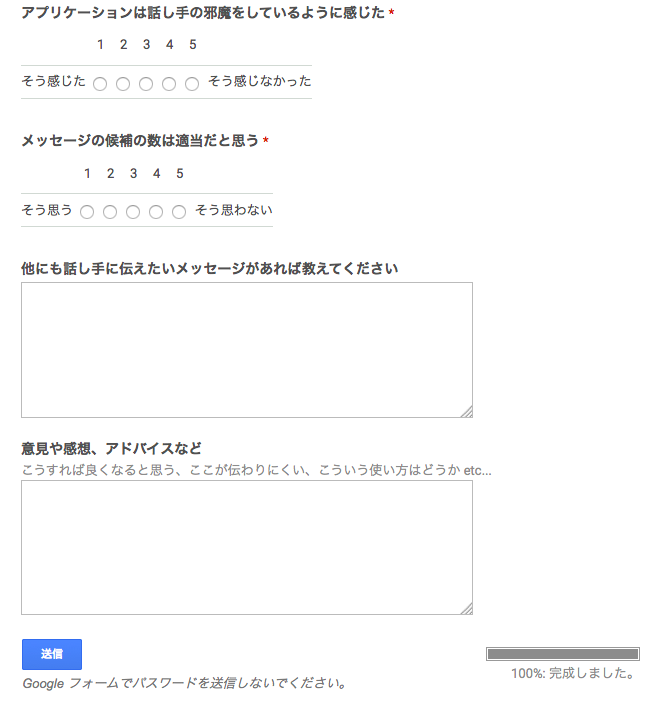
\includegraphics[width=120mm]{./img/ank3.png}
 \end{center}
 \caption{使用したアンケート3}
 \label{leap}
\end{figure}


%--------------------------------------------------------------------
\chapter*{付録その2 Leap Motionを使うための準備}
\subsubsection{Leap Motionを使用するために}
%インストール方法を記述
Leap Motionを使用するために, まず自身のPCにインストーラがインストールされていなければならない. ここではその手順を示す.\\
%置き方、必要なこと、設定方法などを記述
%必要なこと
%インストーラをダウンロード
%解凍 → こうなったらOK

%設定方法
%操作の高さの調節、道具、etc...

%置き方
%パソコンに対して垂直に置くようにする ← 図が必要!!
%注意ごと(一度手をさし出した向きを変えないこと、できるだけ触れないこと)

Leap Motionを使うためには、3つの手順が必要である. 
\begin{enumerate}
 \item インストーラを公式ホームページのセットアップ(図 \ref{setup})からダウンロードする.
 \item ダウンロードしたものを解凍する. 図 \ref{install} のような画面が表示されるので, 指示に従ってインストールする. 
 \item メニューバーにアイコン(図 \ref{setting} )が表示されていたら完了. 
\end{enumerate}

\subsubsection{Leap Motionを使用する前の確認事項}
Leap Motionのアプリケーションを使用する前に確認しておくべきことを2つあげる. 以下に述べることはLeap Motionのアイコン(図 \ref{setting})から設定を選択しLeap Motionの設定画面(図\ref{Lset})から確認することができる. これらの設定後, Visualizer等で確認するとなお良い. \\
 1つは, 操作の高さを調節しておくことである. Leap Motionでは自動調節機能があり, 操作の高さが可変になるが, 初めてLeap Motion使うとこれに気づきにくい. 実際に使ってもらい, 手が疲れるという声があった. ユーザーによって使いやすさに違いが出るので確認しておくべきである. \\
 もう1つは, 道具の設定がオフになっているかどうかを確認することである. Leap Motionではペンなど棒状の道具を検知できる. 今回のアプリケーションでは, 道具を使って操作することを想定しなかったため, 道具の検知を行っていない. もし, 道具を使ってのアプリケーションを製作する場合では, チェックされていないと検知できないため確認する必要がある. \\

\subsubsection{Leap MotionSDKのダウンロード}
Leap Motionを使ったアプリケーションを開発するためにSDKを自分のPCにインストールする必要がある. Leap MotionSDKもLeap Motionインストーラーと同様に, 公式ホームページのセットアップ(図 \ref{setup})よりダウンロードできる. 


\begin{figure}[H]
 \begin{minipage}{0.5\hsize}
  \begin{center}
  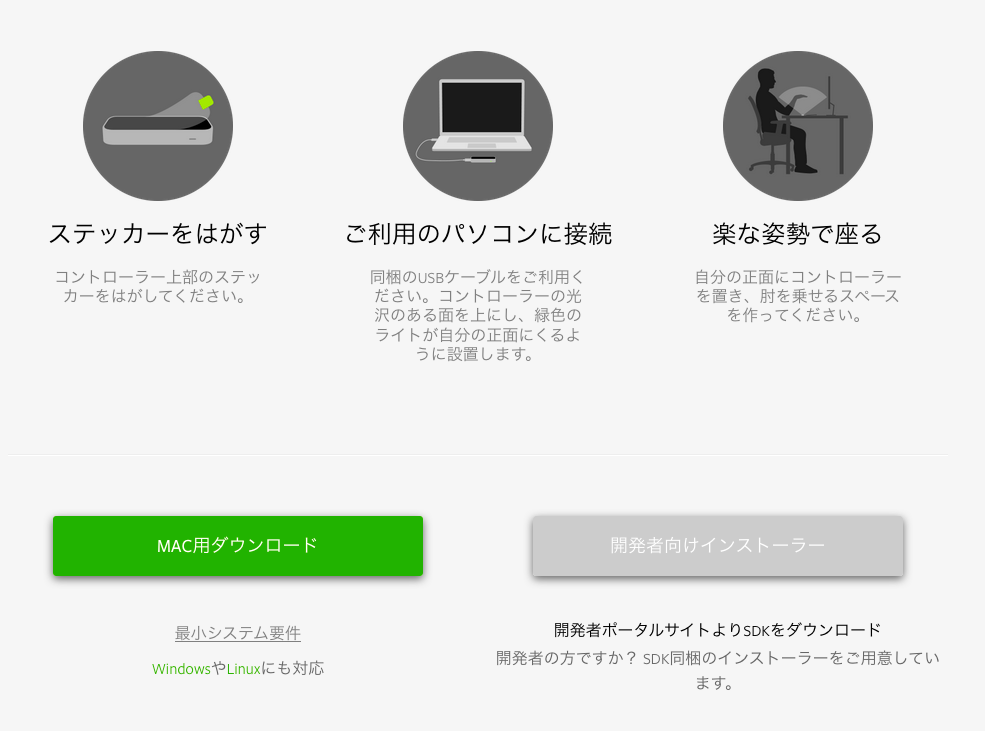
\includegraphics[width=50mm]{./img/setup.png}
  \end{center}
  \caption{Leap Motionのセットアップ}
  \label{setup}
 \end{minipage}
 \begin{minipage}{0.5\hsize}
  \begin{center}
  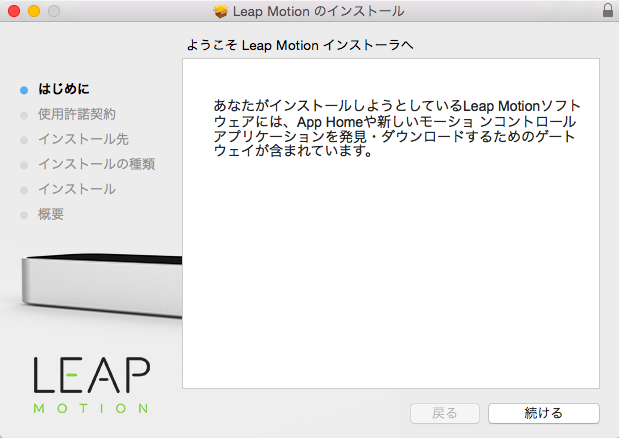
\includegraphics[width=50mm]{./img/installer.png}
  \end{center}
  \caption{インストール画面}
  \label{install}
  \end{minipage}
\end{figure}

\begin{figure}[H]
 \begin{minipage}{0.5\hsize}
  \begin{center}
  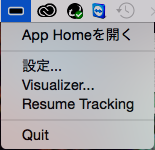
\includegraphics[width=50mm]{./img/setting.png}
  \end{center}
  \caption{Leap Motionのアイコン}
  \label{setting}
 \end{minipage}
 \begin{minipage}{0.5\hsize}
  \begin{center}
  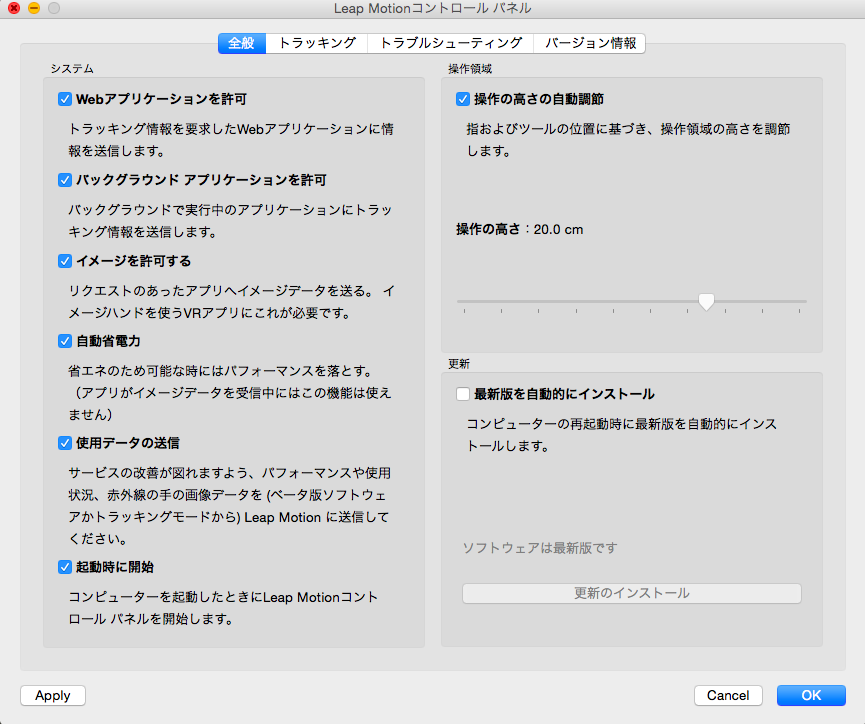
\includegraphics[width=50mm]{./img/Lset.png}
  \end{center}
  \caption{Leap Motionの設定画面}
  \label{Lset}
 \end{minipage}
\end{figure}



%--------------------------------------------------------------------
% 図一覧
\listoffigures

%--------------------------------------------------------------------
% 表一覧
\listoftables

\end{document}